
\documentclass[letterpaper,fleqn,12pt]{article}
%%%%%%%%%%%%%%%%%%%%%%%%%%%%%%%%%%%%%%%%%%%%%%%%%%%%%%%%%%%%%%%%%%%%%%%%%%%%%%%%%%%%%%%%%%%%%%%%%%%%%%%%%%%%%%%%%%%%%%%%%%%%%%%%%%%%%%%%%%%%%%%%%%%%%%%%%%%%%%%%%%%%%%%%%%%%%%%%%%%%%%%%%%%%%%%%%%%%%%%%%%%%%%%%%%%%%%%%%%%%%%%%%%%%%%%%%%%%%%%%%%%%%%%%%%%%
\usepackage{geometry}
\usepackage[singlespacing]{setspace}
\usepackage{amsfonts}
\usepackage{inputenc}
\usepackage{graphicx}
\usepackage{amsmath}
\usepackage{accents}
\usepackage{eurosym}
\usepackage{amssymb}
\usepackage{rotating}
\usepackage{sectsty}
\usepackage{endnotes}
\usepackage{chbibref}
\usepackage{float}
\usepackage{nopageno}
\usepackage[labelsep=period]{caption}
\usepackage{scalefnt}
\usepackage{ragged2e}

\setcounter{MaxMatrixCols}{10}
%TCIDATA{OutputFilter=LATEX.DLL}
%TCIDATA{Version=5.50.0.2953}
%TCIDATA{<META NAME="SaveForMode" CONTENT="2">}
%TCIDATA{BibliographyScheme=Manual}
%TCIDATA{Created=Wednesday, April 07, 2010 09:52:31}
%TCIDATA{LastRevised=Saturday, April 14, 2018 19:56:43}
%TCIDATA{<META NAME="GraphicsSave" CONTENT="32">}
%TCIDATA{<META NAME="DocumentShell" CONTENT="Standard LaTeX\Blank - Standard LaTeX Article">}
%TCIDATA{Language=American English}
%TCIDATA{CSTFile=40 LaTeX article.cst}

\newtheorem{theorem}{Theorem}
\newtheorem{acknowledgement}[theorem]{Acknowledgement}
\newtheorem{algorithm}[theorem]{Algorithm}
\newtheorem{axiom}[theorem]{Axiom}
\newtheorem{case}[theorem]{Case}
\newtheorem{claim}[theorem]{Claim}
\newtheorem{conclusion}[theorem]{Conclusion}
\newtheorem{condition}[theorem]{Condition}
\newtheorem{conjecture}[theorem]{Conjecture}
\newtheorem{corollary}[theorem]{Corollary}
\newtheorem{criterion}[theorem]{Criterion}
\newtheorem{definition}[theorem]{Definition}
\newtheorem{example}[theorem]{Example}
\newtheorem{exercise}[theorem]{Exercise}
\newtheorem{lemma}[theorem]{Lemma}
\newtheorem{notation}[theorem]{Notation}
\newtheorem{problem}[theorem]{Problem}
\newtheorem{proposition}[theorem]{Proposition}
\newtheorem{remark}[theorem]{Remark}
\newtheorem{solution}[theorem]{Solution}
\newtheorem{summary}[theorem]{Summary}
\newenvironment{proof}[1][Proof]{\noindent\textbf{#1.} }{\ \rule{0.5em}{0.5em}}
\geometry{left=1 in,right=1 in,top=1 in,bottom=1 in}
% Macros for Scientific Word 2.5 documents saved with the LaTeX filter.
%Copyright (C) 1994-95 TCI Software Research, Inc.
\typeout{TCILATEX Macros for Scientific Word 2.5 <22 Dec 95>.}
\typeout{NOTICE:  This macro file is NOT proprietary and may be 
freely copied and distributed.}
%
\makeatletter
%
%%%%%%%%%%%%%%%%%%%%%%
% macros for time
\newcount\@hour\newcount\@minute\chardef\@x10\chardef\@xv60
\def\tcitime{
\def\@time{%
  \@minute\time\@hour\@minute\divide\@hour\@xv
  \ifnum\@hour<\@x 0\fi\the\@hour:%
  \multiply\@hour\@xv\advance\@minute-\@hour
  \ifnum\@minute<\@x 0\fi\the\@minute
  }}%

%%%%%%%%%%%%%%%%%%%%%%
% macro for hyperref
\@ifundefined{hyperref}{\def\hyperref#1#2#3#4{#2\ref{#4}#3}}{}

% macro for external program call
\@ifundefined{qExtProgCall}{\def\qExtProgCall#1#2#3#4#5#6{\relax}}{}
%%%%%%%%%%%%%%%%%%%%%%
%
% macros for graphics
%
\def\FILENAME#1{#1}%
%
\def\QCTOpt[#1]#2{%
  \def\QCTOptB{#1}
  \def\QCTOptA{#2}
}
\def\QCTNOpt#1{%
  \def\QCTOptA{#1}
  \let\QCTOptB\empty
}
\def\Qct{%
  \@ifnextchar[{%
    \QCTOpt}{\QCTNOpt}
}
\def\QCBOpt[#1]#2{%
  \def\QCBOptB{#1}
  \def\QCBOptA{#2}
}
\def\QCBNOpt#1{%
  \def\QCBOptA{#1}
  \let\QCBOptB\empty
}
\def\Qcb{%
  \@ifnextchar[{%
    \QCBOpt}{\QCBNOpt}
}
\def\PrepCapArgs{%
  \ifx\QCBOptA\empty
    \ifx\QCTOptA\empty
      {}%
    \else
      \ifx\QCTOptB\empty
        {\QCTOptA}%
      \else
        [\QCTOptB]{\QCTOptA}%
      \fi
    \fi
  \else
    \ifx\QCBOptA\empty
      {}%
    \else
      \ifx\QCBOptB\empty
        {\QCBOptA}%
      \else
        [\QCBOptB]{\QCBOptA}%
      \fi
    \fi
  \fi
}
\newcount\GRAPHICSTYPE
%\GRAPHICSTYPE 0 is for TurboTeX
%\GRAPHICSTYPE 1 is for DVIWindo (PostScript)
%%%(removed)%\GRAPHICSTYPE 2 is for psfig (PostScript)
\GRAPHICSTYPE=\z@
\def\GRAPHICSPS#1{%
 \ifcase\GRAPHICSTYPE%\GRAPHICSTYPE=0
   \special{ps: #1}%
 \or%\GRAPHICSTYPE=1
   \special{language "PS", include "#1"}%
%%%\or%\GRAPHICSTYPE=2
%%%  #1%
 \fi
}%
%
\def\GRAPHICSHP#1{\special{include #1}}%
%
% \graffile{ body }                                  %#1
%          { contentswidth (scalar)  }               %#2
%          { contentsheight (scalar) }               %#3
%          { vertical shift when in-line (scalar) }  %#4
\def\graffile#1#2#3#4{%
%%% \ifnum\GRAPHICSTYPE=\tw@
%%%  %Following if using psfig
%%%  \@ifundefined{psfig}{\input psfig.tex}{}%
%%%  \psfig{file=#1, height=#3, width=#2}%
%%% \else
  %Following for all others
  % JCS - added BOXTHEFRAME, see below
    \leavevmode
    \raise -#4 \BOXTHEFRAME{%
        \hbox to #2{\raise #3\hbox to #2{\null #1\hfil}}}%
}%
%
% A box for drafts
\def\draftbox#1#2#3#4{%
 \leavevmode\raise -#4 \hbox{%
  \frame{\rlap{\protect\tiny #1}\hbox to #2%
   {\vrule height#3 width\z@ depth\z@\hfil}%
  }%
 }%
}%
%
\newcount\draft
\draft=\z@
\let\nographics=\draft
\newif\ifwasdraft
\wasdraftfalse

%  \GRAPHIC{ body }                                  %#1
%          { draft name }                            %#2
%          { contentswidth (scalar)  }               %#3
%          { contentsheight (scalar) }               %#4
%          { vertical shift when in-line (scalar) }  %#5
\def\GRAPHIC#1#2#3#4#5{%
 \ifnum\draft=\@ne\draftbox{#2}{#3}{#4}{#5}%
  \else\graffile{#1}{#3}{#4}{#5}%
  \fi
 }%
%
\def\addtoLaTeXparams#1{%
    \edef\LaTeXparams{\LaTeXparams #1}}%
%
% JCS -  added a switch BoxFrame that can 
% be set by including X in the frame params.
% If set a box is drawn around the frame.

\newif\ifBoxFrame \BoxFramefalse
\newif\ifOverFrame \OverFramefalse
\newif\ifUnderFrame \UnderFramefalse

\def\BOXTHEFRAME#1{%
   \hbox{%
      \ifBoxFrame
         \frame{#1}%
      \else
         {#1}%
      \fi
   }%
}


\def\doFRAMEparams#1{\BoxFramefalse\OverFramefalse\UnderFramefalse\readFRAMEparams#1\end}%
\def\readFRAMEparams#1{%
 \ifx#1\end%
  \let\next=\relax
  \else
  \ifx#1i\dispkind=\z@\fi
  \ifx#1d\dispkind=\@ne\fi
  \ifx#1f\dispkind=\tw@\fi
  \ifx#1t\addtoLaTeXparams{t}\fi
  \ifx#1b\addtoLaTeXparams{b}\fi
  \ifx#1p\addtoLaTeXparams{p}\fi
  \ifx#1h\addtoLaTeXparams{h}\fi
  \ifx#1X\BoxFrametrue\fi
  \ifx#1O\OverFrametrue\fi
  \ifx#1U\UnderFrametrue\fi
  \ifx#1w
    \ifnum\draft=1\wasdrafttrue\else\wasdraftfalse\fi
    \draft=\@ne
  \fi
  \let\next=\readFRAMEparams
  \fi
 \next
 }%
%
%Macro for In-line graphics object
%   \IFRAME{ contentswidth (scalar)  }               %#1
%          { contentsheight (scalar) }               %#2
%          { vertical shift when in-line (scalar) }  %#3
%          { draft name }                            %#4
%          { body }                                  %#5
%          { caption}                                %#6


\def\IFRAME#1#2#3#4#5#6{%
      \bgroup
      \let\QCTOptA\empty
      \let\QCTOptB\empty
      \let\QCBOptA\empty
      \let\QCBOptB\empty
      #6%
      \parindent=0pt%
      \leftskip=0pt
      \rightskip=0pt
      \setbox0 = \hbox{\QCBOptA}%
      \@tempdima = #1\relax
      \ifOverFrame
          % Do this later
          \typeout{This is not implemented yet}%
          \show\HELP
      \else
         \ifdim\wd0>\@tempdima
            \advance\@tempdima by \@tempdima
            \ifdim\wd0 >\@tempdima
               \textwidth=\@tempdima
               \setbox1 =\vbox{%
                  \noindent\hbox to \@tempdima{\hfill\GRAPHIC{#5}{#4}{#1}{#2}{#3}\hfill}\\%
                  \noindent\hbox to \@tempdima{\parbox[b]{\@tempdima}{\QCBOptA}}%
               }%
               \wd1=\@tempdima
            \else
               \textwidth=\wd0
               \setbox1 =\vbox{%
                 \noindent\hbox to \wd0{\hfill\GRAPHIC{#5}{#4}{#1}{#2}{#3}\hfill}\\%
                 \noindent\hbox{\QCBOptA}%
               }%
               \wd1=\wd0
            \fi
         \else
            %\show\BBB
            \ifdim\wd0>0pt
              \hsize=\@tempdima
              \setbox1 =\vbox{%
                \unskip\GRAPHIC{#5}{#4}{#1}{#2}{0pt}%
                \break
                \unskip\hbox to \@tempdima{\hfill \QCBOptA\hfill}%
              }%
              \wd1=\@tempdima
           \else
              \hsize=\@tempdima
              \setbox1 =\vbox{%
                \unskip\GRAPHIC{#5}{#4}{#1}{#2}{0pt}%
              }%
              \wd1=\@tempdima
           \fi
         \fi
         \@tempdimb=\ht1
         \advance\@tempdimb by \dp1
         \advance\@tempdimb by -#2%
         \advance\@tempdimb by #3%
         \leavevmode
         \raise -\@tempdimb \hbox{\box1}%
      \fi
      \egroup%
}%
%
%Macro for Display graphics object
%   \DFRAME{ contentswidth (scalar)  }               %#1
%          { contentsheight (scalar) }               %#2
%          { draft label }                           %#3
%          { name }                                  %#4
%          { caption}                                %#5
\def\DFRAME#1#2#3#4#5{%
 \begin{center}
     \let\QCTOptA\empty
     \let\QCTOptB\empty
     \let\QCBOptA\empty
     \let\QCBOptB\empty
     \ifOverFrame 
        #5\QCTOptA\par
     \fi
     \GRAPHIC{#4}{#3}{#1}{#2}{\z@}
     \ifUnderFrame 
        \nobreak\par #5\QCBOptA
     \fi
 \end{center}%
 }%
%
%Macro for Floating graphic object
%   \FFRAME{ framedata f|i tbph x F|T }              %#1
%          { contentswidth (scalar)  }               %#2
%          { contentsheight (scalar) }               %#3
%          { caption }                               %#4
%          { label }                                 %#5
%          { draft name }                            %#6
%          { body }                                  %#7
\def\FFRAME#1#2#3#4#5#6#7{%
 \begin{figure}[#1]%
  \let\QCTOptA\empty
  \let\QCTOptB\empty
  \let\QCBOptA\empty
  \let\QCBOptB\empty
  \ifOverFrame
    #4
    \ifx\QCTOptA\empty
    \else
      \ifx\QCTOptB\empty
        \caption{\QCTOptA}%
      \else
        \caption[\QCTOptB]{\QCTOptA}%
      \fi
    \fi
    \ifUnderFrame\else
      \label{#5}%
    \fi
  \else
    \UnderFrametrue%
  \fi
  \begin{center}\GRAPHIC{#7}{#6}{#2}{#3}{\z@}\end{center}%
  \ifUnderFrame
    #4
    \ifx\QCBOptA\empty
      \caption{}%
    \else
      \ifx\QCBOptB\empty
        \caption{\QCBOptA}%
      \else
        \caption[\QCBOptB]{\QCBOptA}%
      \fi
    \fi
    \label{#5}%
  \fi
  \end{figure}%
 }%
%
%
%    \FRAME{ framedata f|i tbph x F|T }              %#1
%          { contentswidth (scalar)  }               %#2
%          { contentsheight (scalar) }               %#3
%          { vertical shift when in-line (scalar) }  %#4
%          { caption }                               %#5
%          { label }                                 %#6
%          { name }                                  %#7
%          { body }                                  %#8
%
%    framedata is a string which can contain the following
%    characters: idftbphxFT
%    Their meaning is as follows:
%             i, d or f : in-line, display, or floating
%             t,b,p,h   : LaTeX floating placement options
%             x         : fit contents box to contents
%             F or T    : Figure or Table. 
%                         Later this can expand
%                         to a more general float class.
%
%
\newcount\dispkind%

\def\makeactives{
  \catcode`\"=\active
  \catcode`\;=\active
  \catcode`\:=\active
  \catcode`\'=\active
  \catcode`\~=\active
}
\bgroup
   \makeactives
   \gdef\activesoff{%
      \def"{\string"}
      \def;{\string;}
      \def:{\string:}
      \def'{\string'}
      \def~{\string~}
      %\bbl@deactivate{"}%
      %\bbl@deactivate{;}%
      %\bbl@deactivate{:}%
      %\bbl@deactivate{'}%
    }
\egroup

\def\FRAME#1#2#3#4#5#6#7#8{%
 \bgroup
 \@ifundefined{bbl@deactivate}{}{\activesoff}
 \ifnum\draft=\@ne
   \wasdrafttrue
 \else
   \wasdraftfalse%
 \fi
 \def\LaTeXparams{}%
 \dispkind=\z@
 \def\LaTeXparams{}%
 \doFRAMEparams{#1}%
 \ifnum\dispkind=\z@\IFRAME{#2}{#3}{#4}{#7}{#8}{#5}\else
  \ifnum\dispkind=\@ne\DFRAME{#2}{#3}{#7}{#8}{#5}\else
   \ifnum\dispkind=\tw@
    \edef\@tempa{\noexpand\FFRAME{\LaTeXparams}}%
    \@tempa{#2}{#3}{#5}{#6}{#7}{#8}%
    \fi
   \fi
  \fi
  \ifwasdraft\draft=1\else\draft=0\fi{}%
  \egroup
 }%
%
% This macro added to let SW gobble a parameter that
% should not be passed on and expanded. 

\def\TEXUX#1{"texux"}

%
% Macros for text attributes:
%
\def\BF#1{{\bf {#1}}}%
\def\NEG#1{\leavevmode\hbox{\rlap{\thinspace/}{$#1$}}}%
%
%%%%%%%%%%%%%%%%%%%%%%%%%%%%%%%%%%%%%%%%%%%%%%%%%%%%%%%%%%%%%%%%%%%%%%%%
%
%
% macros for user - defined functions
\def\func#1{\mathop{\rm #1}}%
\def\limfunc#1{\mathop{\rm #1}}%

%
% miscellaneous 
%\long\def\QQQ#1#2{}%
\long\def\QQQ#1#2{%
     \long\expandafter\def\csname#1\endcsname{#2}}%
%\def\QTP#1{}% JCS - this was changed becuase style editor will define QTP
\@ifundefined{QTP}{\def\QTP#1{}}{}
\@ifundefined{QEXCLUDE}{\def\QEXCLUDE#1{}}{}
%\@ifundefined{Qcb}{\def\Qcb#1{#1}}{}
%\@ifundefined{Qct}{\def\Qct#1{#1}}{}
\@ifundefined{Qlb}{\def\Qlb#1{#1}}{}
\@ifundefined{Qlt}{\def\Qlt#1{#1}}{}
\def\QWE{}%
\long\def\QQA#1#2{}%
%\def\QTR#1#2{{\em #2}}% Always \em!!!
%\def\QTR#1#2{\mbox{\begin{#1}#2\end{#1}}}%cb%%%
\def\QTR#1#2{{\csname#1\endcsname #2}}%(gp) Is this the best?
\long\def\TeXButton#1#2{#2}%
\long\def\QSubDoc#1#2{#2}%
\def\EXPAND#1[#2]#3{}%
\def\NOEXPAND#1[#2]#3{}%
\def\PROTECTED{}%
\def\LaTeXparent#1{}%
\def\ChildStyles#1{}%
\def\ChildDefaults#1{}%
\def\QTagDef#1#2#3{}%
%
% Macros for style editor docs
\@ifundefined{StyleEditBeginDoc}{\def\StyleEditBeginDoc{\relax}}{}
%
% Macros for footnotes
\def\QQfnmark#1{\footnotemark}
\def\QQfntext#1#2{\addtocounter{footnote}{#1}\footnotetext{#2}}
%
% Macros for indexing.
\def\MAKEINDEX{\makeatletter\input gnuindex.sty\makeatother\makeindex}%	
\@ifundefined{INDEX}{\def\INDEX#1#2{}{}}{}%
\@ifundefined{SUBINDEX}{\def\SUBINDEX#1#2#3{}{}{}}{}%
\@ifundefined{initial}%  
   {\def\initial#1{\bigbreak{\raggedright\large\bf #1}\kern 2\p@\penalty3000}}%
   {}%
\@ifundefined{entry}{\def\entry#1#2{\item {#1}, #2}}{}%
\@ifundefined{primary}{\def\primary#1{\item {#1}}}{}%
\@ifundefined{secondary}{\def\secondary#1#2{\subitem {#1}, #2}}{}%
%
%
\@ifundefined{ZZZ}{}{\MAKEINDEX\makeatletter}%
%
% Attempts to avoid problems with other styles
\@ifundefined{abstract}{%
 \def\abstract{%
  \if@twocolumn
   \section*{Abstract (Not appropriate in this style!)}%
   \else \small 
   \begin{center}{\bf Abstract\vspace{-.5em}\vspace{\z@}}\end{center}%
   \quotation 
   \fi
  }%
 }{%
 }%
\@ifundefined{endabstract}{\def\endabstract
  {\if@twocolumn\else\endquotation\fi}}{}%
\@ifundefined{maketitle}{\def\maketitle#1{}}{}%
\@ifundefined{affiliation}{\def\affiliation#1{}}{}%
\@ifundefined{proof}{\def\proof{\noindent{\bfseries Proof. }}}{}%
\@ifundefined{endproof}{\def\endproof{\mbox{\ \rule{.1in}{.1in}}}}{}%
\@ifundefined{newfield}{\def\newfield#1#2{}}{}%
\@ifundefined{chapter}{\def\chapter#1{\par(Chapter head:)#1\par }%
 \newcount\c@chapter}{}%
\@ifundefined{part}{\def\part#1{\par(Part head:)#1\par }}{}%
\@ifundefined{section}{\def\section#1{\par(Section head:)#1\par }}{}%
\@ifundefined{subsection}{\def\subsection#1%
 {\par(Subsection head:)#1\par }}{}%
\@ifundefined{subsubsection}{\def\subsubsection#1%
 {\par(Subsubsection head:)#1\par }}{}%
\@ifundefined{paragraph}{\def\paragraph#1%
 {\par(Subsubsubsection head:)#1\par }}{}%
\@ifundefined{subparagraph}{\def\subparagraph#1%
 {\par(Subsubsubsubsection head:)#1\par }}{}%
%%%%%%%%%%%%%%%%%%%%%%%%%%%%%%%%%%%%%%%%%%%%%%%%%%%%%%%%%%%%%%%%%%%%%%%%
% These symbols are not recognized by LaTeX
\@ifundefined{therefore}{\def\therefore{}}{}%
\@ifundefined{backepsilon}{\def\backepsilon{}}{}%
\@ifundefined{yen}{\def\yen{\hbox{\rm\rlap=Y}}}{}%
\@ifundefined{registered}{%
   \def\registered{\relax\ifmmode{}\r@gistered
                    \else$\m@th\r@gistered$\fi}%
 \def\r@gistered{^{\ooalign
  {\hfil\raise.07ex\hbox{$\scriptstyle\rm\text{R}$}\hfil\crcr
  \mathhexbox20D}}}}{}%
\@ifundefined{Eth}{\def\Eth{}}{}%
\@ifundefined{eth}{\def\eth{}}{}%
\@ifundefined{Thorn}{\def\Thorn{}}{}%
\@ifundefined{thorn}{\def\thorn{}}{}%
% A macro to allow any symbol that requires math to appear in text
\def\TEXTsymbol#1{\mbox{$#1$}}%
\@ifundefined{degree}{\def\degree{{}^{\circ}}}{}%
%
% macros for T3TeX files
\newdimen\theight
\def\Column{%
 \vadjust{\setbox\z@=\hbox{\scriptsize\quad\quad tcol}%
  \theight=\ht\z@\advance\theight by \dp\z@\advance\theight by \lineskip
  \kern -\theight \vbox to \theight{%
   \rightline{\rlap{\box\z@}}%
   \vss
   }%
  }%
 }%
%
\def\qed{%
 \ifhmode\unskip\nobreak\fi\ifmmode\ifinner\else\hskip5\p@\fi\fi
 \hbox{\hskip5\p@\vrule width4\p@ height6\p@ depth1.5\p@\hskip\p@}%
 }%
%
\def\cents{\hbox{\rm\rlap/c}}%
\def\miss{\hbox{\vrule height2\p@ width 2\p@ depth\z@}}%
%\def\miss{\hbox{.}}%        %another possibility 
%
\def\vvert{\Vert}%           %always translated to \left| or \right|
%
\def\tcol#1{{\baselineskip=6\p@ \vcenter{#1}} \Column}  %
%
\def\dB{\hbox{{}}}%                 %dummy entry in column 
\def\mB#1{\hbox{$#1$}}%             %column entry
\def\nB#1{\hbox{#1}}%               %column entry (not math)
%
%\newcount\notenumber
%\def\clearnotenumber{\notenumber=0}
%\def\note{\global\advance\notenumber by 1
% \footnote{$^{\the\notenumber}$}}
%\def\note{\global\advance\notenumber by 1
\def\note{$^{\dag}}%
%
%

\def\newfmtname{LaTeX2e}
\def\chkcompat{%
   \if@compatibility
   \else
     \usepackage{latexsym}
   \fi
}

\ifx\fmtname\newfmtname
  \DeclareOldFontCommand{\rm}{\normalfont\rmfamily}{\mathrm}
  \DeclareOldFontCommand{\sf}{\normalfont\sffamily}{\mathsf}
  \DeclareOldFontCommand{\tt}{\normalfont\ttfamily}{\mathtt}
  \DeclareOldFontCommand{\bf}{\normalfont\bfseries}{\mathbf}
  \DeclareOldFontCommand{\it}{\normalfont\itshape}{\mathit}
  \DeclareOldFontCommand{\sl}{\normalfont\slshape}{\@nomath\sl}
  \DeclareOldFontCommand{\sc}{\normalfont\scshape}{\@nomath\sc}
  \chkcompat
\fi

%
% Greek bold macros
% Redefine all of the math symbols 
% which might be bolded	 - there are 
% probably others to add to this list

\def\alpha{\Greekmath 010B }%
\def\beta{\Greekmath 010C }%
\def\gamma{\Greekmath 010D }%
\def\delta{\Greekmath 010E }%
\def\epsilon{\Greekmath 010F }%
\def\zeta{\Greekmath 0110 }%
\def\eta{\Greekmath 0111 }%
\def\theta{\Greekmath 0112 }%
\def\iota{\Greekmath 0113 }%
\def\kappa{\Greekmath 0114 }%
\def\lambda{\Greekmath 0115 }%
\def\mu{\Greekmath 0116 }%
\def\nu{\Greekmath 0117 }%
\def\xi{\Greekmath 0118 }%
\def\pi{\Greekmath 0119 }%
\def\rho{\Greekmath 011A }%
\def\sigma{\Greekmath 011B }%
\def\tau{\Greekmath 011C }%
\def\upsilon{\Greekmath 011D }%
\def\phi{\Greekmath 011E }%
\def\chi{\Greekmath 011F }%
\def\psi{\Greekmath 0120 }%
\def\omega{\Greekmath 0121 }%
\def\varepsilon{\Greekmath 0122 }%
\def\vartheta{\Greekmath 0123 }%
\def\varpi{\Greekmath 0124 }%
\def\varrho{\Greekmath 0125 }%
\def\varsigma{\Greekmath 0126 }%
\def\varphi{\Greekmath 0127 }%

\def\nabla{\Greekmath 0272 }
\def\FindBoldGroup{%
   {\setbox0=\hbox{$\mathbf{x\global\edef\theboldgroup{\the\mathgroup}}$}}%
}

\def\Greekmath#1#2#3#4{%
    \if@compatibility
        \ifnum\mathgroup=\symbold
           \mathchoice{\mbox{\boldmath$\displaystyle\mathchar"#1#2#3#4$}}%
                      {\mbox{\boldmath$\textstyle\mathchar"#1#2#3#4$}}%
                      {\mbox{\boldmath$\scriptstyle\mathchar"#1#2#3#4$}}%
                      {\mbox{\boldmath$\scriptscriptstyle\mathchar"#1#2#3#4$}}%
        \else
           \mathchar"#1#2#3#4% 
        \fi 
    \else 
        \FindBoldGroup
        \ifnum\mathgroup=\theboldgroup % For 2e
           \mathchoice{\mbox{\boldmath$\displaystyle\mathchar"#1#2#3#4$}}%
                      {\mbox{\boldmath$\textstyle\mathchar"#1#2#3#4$}}%
                      {\mbox{\boldmath$\scriptstyle\mathchar"#1#2#3#4$}}%
                      {\mbox{\boldmath$\scriptscriptstyle\mathchar"#1#2#3#4$}}%
        \else
           \mathchar"#1#2#3#4% 
        \fi     	    
	  \fi}

\newif\ifGreekBold  \GreekBoldfalse
\let\SAVEPBF=\pbf
\def\pbf{\GreekBoldtrue\SAVEPBF}%
%

\@ifundefined{theorem}{\newtheorem{theorem}{Theorem}}{}
\@ifundefined{lemma}{\newtheorem{lemma}[theorem]{Lemma}}{}
\@ifundefined{corollary}{\newtheorem{corollary}[theorem]{Corollary}}{}
\@ifundefined{conjecture}{\newtheorem{conjecture}[theorem]{Conjecture}}{}
\@ifundefined{proposition}{\newtheorem{proposition}[theorem]{Proposition}}{}
\@ifundefined{axiom}{\newtheorem{axiom}{Axiom}}{}
\@ifundefined{remark}{\newtheorem{remark}{Remark}}{}
\@ifundefined{example}{\newtheorem{example}{Example}}{}
\@ifundefined{exercise}{\newtheorem{exercise}{Exercise}}{}
\@ifundefined{definition}{\newtheorem{definition}{Definition}}{}


\@ifundefined{mathletters}{%
  %\def\theequation{\arabic{equation}}
  \newcounter{equationnumber}  
  \def\mathletters{%
     \addtocounter{equation}{1}
     \edef\@currentlabel{\theequation}%
     \setcounter{equationnumber}{\c@equation}
     \setcounter{equation}{0}%
     \edef\theequation{\@currentlabel\noexpand\alph{equation}}%
  }
  \def\endmathletters{%
     \setcounter{equation}{\value{equationnumber}}%
  }
}{}

%Logos
\@ifundefined{BibTeX}{%
    \def\BibTeX{{\rm B\kern-.05em{\sc i\kern-.025em b}\kern-.08em
                 T\kern-.1667em\lower.7ex\hbox{E}\kern-.125emX}}}{}%
\@ifundefined{AmS}%
    {\def\AmS{{\protect\usefont{OMS}{cmsy}{m}{n}%
                A\kern-.1667em\lower.5ex\hbox{M}\kern-.125emS}}}{}%
\@ifundefined{AmSTeX}{\def\AmSTeX{\protect\AmS-\protect\TeX\@}}{}%
%

%%%%%%%%%%%%%%%%%%%%%%%%%%%%%%%%%%%%%%%%%%%%%%%%%%%%%%%%%%%%%%%%%%%%%%%
% NOTE: The rest of this file is read only if amstex has not been
% loaded.  This section is used to define amstex constructs in the
% event they have not been defined.
%
%
\ifx\ds@amstex\relax
   \message{amstex already loaded}\makeatother\endinput% 2.09 compatability
\else
   \@ifpackageloaded{amstex}%
      {\message{amstex already loaded}\makeatother\endinput}
      {}
   \@ifpackageloaded{amsgen}%
      {\message{amsgen already loaded}\makeatother\endinput}
      {}
\fi
%%%%%%%%%%%%%%%%%%%%%%%%%%%%%%%%%%%%%%%%%%%%%%%%%%%%%%%%%%%%%%%%%%%%%%%%
%%
%
%
%  Macros to define some AMS LaTeX constructs when 
%  AMS LaTeX has not been loaded
% 
% These macros are copied from the AMS-TeX package for doing
% multiple integrals.
%
\let\DOTSI\relax
\def\RIfM@{\relax\ifmmode}%
\def\FN@{\futurelet\next}%
\newcount\intno@
\def\iint{\DOTSI\intno@\tw@\FN@\ints@}%
\def\iiint{\DOTSI\intno@\thr@@\FN@\ints@}%
\def\iiiint{\DOTSI\intno@4 \FN@\ints@}%
\def\idotsint{\DOTSI\intno@\z@\FN@\ints@}%
\def\ints@{\findlimits@\ints@@}%
\newif\iflimtoken@
\newif\iflimits@
\def\findlimits@{\limtoken@true\ifx\next\limits\limits@true
 \else\ifx\next\nolimits\limits@false\else
 \limtoken@false\ifx\ilimits@\nolimits\limits@false\else
 \ifinner\limits@false\else\limits@true\fi\fi\fi\fi}%
\def\multint@{\int\ifnum\intno@=\z@\intdots@                          %1
 \else\intkern@\fi                                                    %2
 \ifnum\intno@>\tw@\int\intkern@\fi                                   %3
 \ifnum\intno@>\thr@@\int\intkern@\fi                                 %4
 \int}%                                                               %5
\def\multintlimits@{\intop\ifnum\intno@=\z@\intdots@\else\intkern@\fi
 \ifnum\intno@>\tw@\intop\intkern@\fi
 \ifnum\intno@>\thr@@\intop\intkern@\fi\intop}%
\def\intic@{%
    \mathchoice{\hskip.5em}{\hskip.4em}{\hskip.4em}{\hskip.4em}}%
\def\negintic@{\mathchoice
 {\hskip-.5em}{\hskip-.4em}{\hskip-.4em}{\hskip-.4em}}%
\def\ints@@{\iflimtoken@                                              %1
 \def\ints@@@{\iflimits@\negintic@
   \mathop{\intic@\multintlimits@}\limits                             %2
  \else\multint@\nolimits\fi                                          %3
  \eat@}%                                                             %4
 \else                                                                %5
 \def\ints@@@{\iflimits@\negintic@
  \mathop{\intic@\multintlimits@}\limits\else
  \multint@\nolimits\fi}\fi\ints@@@}%
\def\intkern@{\mathchoice{\!\!\!}{\!\!}{\!\!}{\!\!}}%
\def\plaincdots@{\mathinner{\cdotp\cdotp\cdotp}}%
\def\intdots@{\mathchoice{\plaincdots@}%
 {{\cdotp}\mkern1.5mu{\cdotp}\mkern1.5mu{\cdotp}}%
 {{\cdotp}\mkern1mu{\cdotp}\mkern1mu{\cdotp}}%
 {{\cdotp}\mkern1mu{\cdotp}\mkern1mu{\cdotp}}}%
%
%
%  These macros are for doing the AMS \text{} construct
%
\def\RIfM@{\relax\protect\ifmmode}
\def\text{\RIfM@\expandafter\text@\else\expandafter\mbox\fi}
\let\nfss@text\text
\def\text@#1{\mathchoice
   {\textdef@\displaystyle\f@size{#1}}%
   {\textdef@\textstyle\tf@size{\firstchoice@false #1}}%
   {\textdef@\textstyle\sf@size{\firstchoice@false #1}}%
   {\textdef@\textstyle \ssf@size{\firstchoice@false #1}}%
   \glb@settings}

\def\textdef@#1#2#3{\hbox{{%
                    \everymath{#1}%
                    \let\f@size#2\selectfont
                    #3}}}
\newif\iffirstchoice@
\firstchoice@true
%
%    Old Scheme for \text
%
%\def\rmfam{\z@}%
%\newif\iffirstchoice@
%\firstchoice@true
%\def\textfonti{\the\textfont\@ne}%
%\def\textfontii{\the\textfont\tw@}%
%\def\text{\RIfM@\expandafter\text@\else\expandafter\text@@\fi}%
%\def\text@@#1{\leavevmode\hbox{#1}}%
%\def\text@#1{\mathchoice
% {\hbox{\everymath{\displaystyle}\def\textfonti{\the\textfont\@ne}%
%  \def\textfontii{\the\textfont\tw@}\textdef@@ T#1}}%
% {\hbox{\firstchoice@false
%  \everymath{\textstyle}\def\textfonti{\the\textfont\@ne}%
%  \def\textfontii{\the\textfont\tw@}\textdef@@ T#1}}%
% {\hbox{\firstchoice@false
%  \everymath{\scriptstyle}\def\textfonti{\the\scriptfont\@ne}%
%  \def\textfontii{\the\scriptfont\tw@}\textdef@@ S\rm#1}}%
% {\hbox{\firstchoice@false
%  \everymath{\scriptscriptstyle}\def\textfonti
%  {\the\scriptscriptfont\@ne}%
%  \def\textfontii{\the\scriptscriptfont\tw@}\textdef@@ s\rm#1}}}%
%\def\textdef@@#1{\textdef@#1\rm\textdef@#1\bf\textdef@#1\sl
%    \textdef@#1\it}%
%\def\DN@{\def\next@}%
%\def\eat@#1{}%
%\def\textdef@#1#2{%
% \DN@{\csname\expandafter\eat@\string#2fam\endcsname}%
% \if S#1\edef#2{\the\scriptfont\next@\relax}%
% \else\if s#1\edef#2{\the\scriptscriptfont\next@\relax}%
% \else\edef#2{\the\textfont\next@\relax}\fi\fi}%
%
%
%These are the AMS constructs for multiline limits.
%
\def\Let@{\relax\iffalse{\fi\let\\=\cr\iffalse}\fi}%
\def\vspace@{\def\vspace##1{\crcr\noalign{\vskip##1\relax}}}%
\def\multilimits@{\bgroup\vspace@\Let@
 \baselineskip\fontdimen10 \scriptfont\tw@
 \advance\baselineskip\fontdimen12 \scriptfont\tw@
 \lineskip\thr@@\fontdimen8 \scriptfont\thr@@
 \lineskiplimit\lineskip
 \vbox\bgroup\ialign\bgroup\hfil$\m@th\scriptstyle{##}$\hfil\crcr}%
\def\Sb{_\multilimits@}%
\def\endSb{\crcr\egroup\egroup\egroup}%
\def\Sp{^\multilimits@}%
\let\endSp\endSb
%
%
%These are AMS constructs for horizontal arrows
%
\newdimen\ex@
\ex@.2326ex
\def\rightarrowfill@#1{$#1\m@th\mathord-\mkern-6mu\cleaders
 \hbox{$#1\mkern-2mu\mathord-\mkern-2mu$}\hfill
 \mkern-6mu\mathord\rightarrow$}%
\def\leftarrowfill@#1{$#1\m@th\mathord\leftarrow\mkern-6mu\cleaders
 \hbox{$#1\mkern-2mu\mathord-\mkern-2mu$}\hfill\mkern-6mu\mathord-$}%
\def\leftrightarrowfill@#1{$#1\m@th\mathord\leftarrow
\mkern-6mu\cleaders
 \hbox{$#1\mkern-2mu\mathord-\mkern-2mu$}\hfill
 \mkern-6mu\mathord\rightarrow$}%
\def\overrightarrow{\mathpalette\overrightarrow@}%
\def\overrightarrow@#1#2{\vbox{\ialign{##\crcr\rightarrowfill@#1\crcr
 \noalign{\kern-\ex@\nointerlineskip}$\m@th\hfil#1#2\hfil$\crcr}}}%
\let\overarrow\overrightarrow
\def\overleftarrow{\mathpalette\overleftarrow@}%
\def\overleftarrow@#1#2{\vbox{\ialign{##\crcr\leftarrowfill@#1\crcr
 \noalign{\kern-\ex@\nointerlineskip}$\m@th\hfil#1#2\hfil$\crcr}}}%
\def\overleftrightarrow{\mathpalette\overleftrightarrow@}%
\def\overleftrightarrow@#1#2{\vbox{\ialign{##\crcr
   \leftrightarrowfill@#1\crcr
 \noalign{\kern-\ex@\nointerlineskip}$\m@th\hfil#1#2\hfil$\crcr}}}%
\def\underrightarrow{\mathpalette\underrightarrow@}%
\def\underrightarrow@#1#2{\vtop{\ialign{##\crcr$\m@th\hfil#1#2\hfil
  $\crcr\noalign{\nointerlineskip}\rightarrowfill@#1\crcr}}}%
\let\underarrow\underrightarrow
\def\underleftarrow{\mathpalette\underleftarrow@}%
\def\underleftarrow@#1#2{\vtop{\ialign{##\crcr$\m@th\hfil#1#2\hfil
  $\crcr\noalign{\nointerlineskip}\leftarrowfill@#1\crcr}}}%
\def\underleftrightarrow{\mathpalette\underleftrightarrow@}%
\def\underleftrightarrow@#1#2{\vtop{\ialign{##\crcr$\m@th
  \hfil#1#2\hfil$\crcr
 \noalign{\nointerlineskip}\leftrightarrowfill@#1\crcr}}}%
%%%%%%%%%%%%%%%%%%%%%

% 94.0815 by Jon:

\def\qopnamewl@#1{\mathop{\operator@font#1}\nlimits@}
\let\nlimits@\displaylimits
\def\setboxz@h{\setbox\z@\hbox}


\def\varlim@#1#2{\mathop{\vtop{\ialign{##\crcr
 \hfil$#1\m@th\operator@font lim$\hfil\crcr
 \noalign{\nointerlineskip}#2#1\crcr
 \noalign{\nointerlineskip\kern-\ex@}\crcr}}}}

 \def\rightarrowfill@#1{\m@th\setboxz@h{$#1-$}\ht\z@\z@
  $#1\copy\z@\mkern-6mu\cleaders
  \hbox{$#1\mkern-2mu\box\z@\mkern-2mu$}\hfill
  \mkern-6mu\mathord\rightarrow$}
\def\leftarrowfill@#1{\m@th\setboxz@h{$#1-$}\ht\z@\z@
  $#1\mathord\leftarrow\mkern-6mu\cleaders
  \hbox{$#1\mkern-2mu\copy\z@\mkern-2mu$}\hfill
  \mkern-6mu\box\z@$}


\def\projlim{\qopnamewl@{proj\,lim}}
\def\injlim{\qopnamewl@{inj\,lim}}
\def\varinjlim{\mathpalette\varlim@\rightarrowfill@}
\def\varprojlim{\mathpalette\varlim@\leftarrowfill@}
\def\varliminf{\mathpalette\varliminf@{}}
\def\varliminf@#1{\mathop{\underline{\vrule\@depth.2\ex@\@width\z@
   \hbox{$#1\m@th\operator@font lim$}}}}
\def\varlimsup{\mathpalette\varlimsup@{}}
\def\varlimsup@#1{\mathop{\overline
  {\hbox{$#1\m@th\operator@font lim$}}}}

%
%%%%%%%%%%%%%%%%%%%%%%%%%%%%%%%%%%%%%%%%%%%%%%%%%%%%%%%%%%%%%%%%%%%%%
%
\def\tfrac#1#2{{\textstyle {#1 \over #2}}}%
\def\dfrac#1#2{{\displaystyle {#1 \over #2}}}%
\def\binom#1#2{{#1 \choose #2}}%
\def\tbinom#1#2{{\textstyle {#1 \choose #2}}}%
\def\dbinom#1#2{{\displaystyle {#1 \choose #2}}}%
\def\QATOP#1#2{{#1 \atop #2}}%
\def\QTATOP#1#2{{\textstyle {#1 \atop #2}}}%
\def\QDATOP#1#2{{\displaystyle {#1 \atop #2}}}%
\def\QABOVE#1#2#3{{#2 \above#1 #3}}%
\def\QTABOVE#1#2#3{{\textstyle {#2 \above#1 #3}}}%
\def\QDABOVE#1#2#3{{\displaystyle {#2 \above#1 #3}}}%
\def\QOVERD#1#2#3#4{{#3 \overwithdelims#1#2 #4}}%
\def\QTOVERD#1#2#3#4{{\textstyle {#3 \overwithdelims#1#2 #4}}}%
\def\QDOVERD#1#2#3#4{{\displaystyle {#3 \overwithdelims#1#2 #4}}}%
\def\QATOPD#1#2#3#4{{#3 \atopwithdelims#1#2 #4}}%
\def\QTATOPD#1#2#3#4{{\textstyle {#3 \atopwithdelims#1#2 #4}}}%
\def\QDATOPD#1#2#3#4{{\displaystyle {#3 \atopwithdelims#1#2 #4}}}%
\def\QABOVED#1#2#3#4#5{{#4 \abovewithdelims#1#2#3 #5}}%
\def\QTABOVED#1#2#3#4#5{{\textstyle 
   {#4 \abovewithdelims#1#2#3 #5}}}%
\def\QDABOVED#1#2#3#4#5{{\displaystyle 
   {#4 \abovewithdelims#1#2#3 #5}}}%
%
% Macros for text size operators:

%JCS - added braces and \mathop around \displaystyle\int, etc.
%
\def\tint{\mathop{\textstyle \int}}%
\def\tiint{\mathop{\textstyle \iint }}%
\def\tiiint{\mathop{\textstyle \iiint }}%
\def\tiiiint{\mathop{\textstyle \iiiint }}%
\def\tidotsint{\mathop{\textstyle \idotsint }}%
\def\toint{\mathop{\textstyle \oint}}%
\def\tsum{\mathop{\textstyle \sum }}%
\def\tprod{\mathop{\textstyle \prod }}%
\def\tbigcap{\mathop{\textstyle \bigcap }}%
\def\tbigwedge{\mathop{\textstyle \bigwedge }}%
\def\tbigoplus{\mathop{\textstyle \bigoplus }}%
\def\tbigodot{\mathop{\textstyle \bigodot }}%
\def\tbigsqcup{\mathop{\textstyle \bigsqcup }}%
\def\tcoprod{\mathop{\textstyle \coprod }}%
\def\tbigcup{\mathop{\textstyle \bigcup }}%
\def\tbigvee{\mathop{\textstyle \bigvee }}%
\def\tbigotimes{\mathop{\textstyle \bigotimes }}%
\def\tbiguplus{\mathop{\textstyle \biguplus }}%
%
%
%Macros for display size operators:
%

\def\dint{\mathop{\displaystyle \int}}%
\def\diint{\mathop{\displaystyle \iint }}%
\def\diiint{\mathop{\displaystyle \iiint }}%
\def\diiiint{\mathop{\displaystyle \iiiint }}%
\def\didotsint{\mathop{\displaystyle \idotsint }}%
\def\doint{\mathop{\displaystyle \oint}}%
\def\dsum{\mathop{\displaystyle \sum }}%
\def\dprod{\mathop{\displaystyle \prod }}%
\def\dbigcap{\mathop{\displaystyle \bigcap }}%
\def\dbigwedge{\mathop{\displaystyle \bigwedge }}%
\def\dbigoplus{\mathop{\displaystyle \bigoplus }}%
\def\dbigodot{\mathop{\displaystyle \bigodot }}%
\def\dbigsqcup{\mathop{\displaystyle \bigsqcup }}%
\def\dcoprod{\mathop{\displaystyle \coprod }}%
\def\dbigcup{\mathop{\displaystyle \bigcup }}%
\def\dbigvee{\mathop{\displaystyle \bigvee }}%
\def\dbigotimes{\mathop{\displaystyle \bigotimes }}%
\def\dbiguplus{\mathop{\displaystyle \biguplus }}%
%
%Companion to stackrel
\def\stackunder#1#2{\mathrel{\mathop{#2}\limits_{#1}}}%
%
%
% These are AMS environments that will be defined to
% be verbatims if amstex has not actually been 
% loaded
%
%
\begingroup \catcode `|=0 \catcode `[= 1
\catcode`]=2 \catcode `\{=12 \catcode `\}=12
\catcode`\\=12 
|gdef|@alignverbatim#1\end{align}[#1|end[align]]
|gdef|@salignverbatim#1\end{align*}[#1|end[align*]]

|gdef|@alignatverbatim#1\end{alignat}[#1|end[alignat]]
|gdef|@salignatverbatim#1\end{alignat*}[#1|end[alignat*]]

|gdef|@xalignatverbatim#1\end{xalignat}[#1|end[xalignat]]
|gdef|@sxalignatverbatim#1\end{xalignat*}[#1|end[xalignat*]]

|gdef|@gatherverbatim#1\end{gather}[#1|end[gather]]
|gdef|@sgatherverbatim#1\end{gather*}[#1|end[gather*]]

|gdef|@gatherverbatim#1\end{gather}[#1|end[gather]]
|gdef|@sgatherverbatim#1\end{gather*}[#1|end[gather*]]


|gdef|@multilineverbatim#1\end{multiline}[#1|end[multiline]]
|gdef|@smultilineverbatim#1\end{multiline*}[#1|end[multiline*]]

|gdef|@arraxverbatim#1\end{arrax}[#1|end[arrax]]
|gdef|@sarraxverbatim#1\end{arrax*}[#1|end[arrax*]]

|gdef|@tabulaxverbatim#1\end{tabulax}[#1|end[tabulax]]
|gdef|@stabulaxverbatim#1\end{tabulax*}[#1|end[tabulax*]]


|endgroup
  

  
\def\align{\@verbatim \frenchspacing\@vobeyspaces \@alignverbatim
You are using the "align" environment in a style in which it is not defined.}
\let\endalign=\endtrivlist
 
\@namedef{align*}{\@verbatim\@salignverbatim
You are using the "align*" environment in a style in which it is not defined.}
\expandafter\let\csname endalign*\endcsname =\endtrivlist




\def\alignat{\@verbatim \frenchspacing\@vobeyspaces \@alignatverbatim
You are using the "alignat" environment in a style in which it is not defined.}
\let\endalignat=\endtrivlist
 
\@namedef{alignat*}{\@verbatim\@salignatverbatim
You are using the "alignat*" environment in a style in which it is not defined.}
\expandafter\let\csname endalignat*\endcsname =\endtrivlist




\def\xalignat{\@verbatim \frenchspacing\@vobeyspaces \@xalignatverbatim
You are using the "xalignat" environment in a style in which it is not defined.}
\let\endxalignat=\endtrivlist
 
\@namedef{xalignat*}{\@verbatim\@sxalignatverbatim
You are using the "xalignat*" environment in a style in which it is not defined.}
\expandafter\let\csname endxalignat*\endcsname =\endtrivlist




\def\gather{\@verbatim \frenchspacing\@vobeyspaces \@gatherverbatim
You are using the "gather" environment in a style in which it is not defined.}
\let\endgather=\endtrivlist
 
\@namedef{gather*}{\@verbatim\@sgatherverbatim
You are using the "gather*" environment in a style in which it is not defined.}
\expandafter\let\csname endgather*\endcsname =\endtrivlist


\def\multiline{\@verbatim \frenchspacing\@vobeyspaces \@multilineverbatim
You are using the "multiline" environment in a style in which it is not defined.}
\let\endmultiline=\endtrivlist
 
\@namedef{multiline*}{\@verbatim\@smultilineverbatim
You are using the "multiline*" environment in a style in which it is not defined.}
\expandafter\let\csname endmultiline*\endcsname =\endtrivlist


\def\arrax{\@verbatim \frenchspacing\@vobeyspaces \@arraxverbatim
You are using a type of "array" construct that is only allowed in AmS-LaTeX.}
\let\endarrax=\endtrivlist

\def\tabulax{\@verbatim \frenchspacing\@vobeyspaces \@tabulaxverbatim
You are using a type of "tabular" construct that is only allowed in AmS-LaTeX.}
\let\endtabulax=\endtrivlist

 
\@namedef{arrax*}{\@verbatim\@sarraxverbatim
You are using a type of "array*" construct that is only allowed in AmS-LaTeX.}
\expandafter\let\csname endarrax*\endcsname =\endtrivlist

\@namedef{tabulax*}{\@verbatim\@stabulaxverbatim
You are using a type of "tabular*" construct that is only allowed in AmS-LaTeX.}
\expandafter\let\csname endtabulax*\endcsname =\endtrivlist

% macro to simulate ams tag construct


% This macro is a fix to eqnarray
\def\@@eqncr{\let\@tempa\relax
    \ifcase\@eqcnt \def\@tempa{& & &}\or \def\@tempa{& &}%
      \else \def\@tempa{&}\fi
     \@tempa
     \if@eqnsw
        \iftag@
           \@taggnum
        \else
           \@eqnnum\stepcounter{equation}%
        \fi
     \fi
     \global\tag@false
     \global\@eqnswtrue
     \global\@eqcnt\z@\cr}


% This macro is a fix to the equation environment
 \def\endequation{%
     \ifmmode\ifinner % FLEQN hack
      \iftag@
        \addtocounter{equation}{-1} % undo the increment made in the begin part
        $\hfil
           \displaywidth\linewidth\@taggnum\egroup \endtrivlist
        \global\tag@false
        \global\@ignoretrue   
      \else
        $\hfil
           \displaywidth\linewidth\@eqnnum\egroup \endtrivlist
        \global\tag@false
        \global\@ignoretrue 
      \fi
     \else   
      \iftag@
        \addtocounter{equation}{-1} % undo the increment made in the begin part
        \eqno \hbox{\@taggnum}
        \global\tag@false%
        $$\global\@ignoretrue
      \else
        \eqno \hbox{\@eqnnum}% $$ BRACE MATCHING HACK
        $$\global\@ignoretrue
      \fi
     \fi\fi
 } 

 \newif\iftag@ \tag@false
 
 \def\tag{\@ifnextchar*{\@tagstar}{\@tag}}
 \def\@tag#1{%
     \global\tag@true
     \global\def\@taggnum{(#1)}}
 \def\@tagstar*#1{%
     \global\tag@true
     \global\def\@taggnum{#1}%  
}

% Do not add anything to the end of this file.  
% The last section of the file is loaded only if 
% amstex has not been.



\makeatother
\endinput

\setlength{\abovecaptionskip}{4pt}
\makeatletter
\def\@biblabel#1{\hspace*{-\labelsep}}
\newdimen\@bibhang \@bibhang=2em
\def\setbibhang#1{\@bibhang=#1}
\renewenvironment{thebibliography}[1]{  \setlength{\labelwidth}{0pt}
  \setlength{\labelsep}{0pt}
  \section*{\refname
     \@mkboth{\uppercase{\refname}}{\uppercase{\refname}}}   \vspace{0em}
   \setlength{\parindent}{0pt}
   \def\newblock{}
   \renewcommand{\bibitem}[2][]{     \if@filesw
       {\let\protect\noexpand\immediate
        \write\@auxout{\string\bibcite{##2}{##1}}}
        \fi\hangindent=\@bibhang\hangafter=1}}
\makeatother

\begin{document}

\title{Estimation of nested and zero-inflated ordered probit models\\
\bigskip }
\date{}
\author{David Dale \\
%EndAName
Yandex\\
Moscow, Russia\\
dale.david@yandex.ru \and Andrei Sirchenko \\
%EndAName
Higher School of Economics\\
Moscow, Russia\\
andrei.sirchenko@gmail.com}
\maketitle

\begin{abstract}
We present the STATA commands, \texttt{nop}, \texttt{ziop-2} and \texttt{%
ziop-3}, which estimate the three-part nested ordered probit model, the
two-part cross-nested zero-inflated ordered probit models of Harris and Zhao
(2007, \textit{Journal of Econometrics }141(2): 1073--1099) and Brooks,
Harris and Spencer (2012,\ \textit{Economics Letters} 117(3): 683--686), and
the three-part cross-nested zero-inflated ordered probit model, with both
exogenous and endogenous switching. The zero-inflated models address the
inflation of neutral (zero) observations and allows the zeros to emerge in
two or three latent regimes. The three-part models also allow the
probabilities of positive and negative outcomes to be generated by distinct
processes. We investigate the finite-sample performance of proposed maximum
likelihood estimators by Monte Carlo simulations, and illustrate the models
with an empirical application to federal funds rate target.

\bigskip \bigskip \bigskip \bigskip \bigskip \bigskip \bigskip

\bigskip \bigskip \bigskip \bigskip \bigskip \bigskip \bigskip

\bigskip \bigskip \bigskip \bigskip \bigskip \bigskip \bigskip

\textbf{Keywords:} ordinal responses, nested ordered probit, zero inflation,
endogenous switching, Monte Carlo simulation, federal funds rate target.

\bigskip \bigskip \bigskip \bigskip \bigskip
\end{abstract}

%TCIMACRO{\TeXButton{Onehalf}{\begin{onehalfspace}}}%
%BeginExpansion
\begin{onehalfspace}%
%EndExpansion

\section{Introduction}

We introduce the STATA\ commands, \texttt{nop}, \texttt{ziop-2} and \texttt{%
ziop-3}, which estimate the two-level nested and cross-nested ordered-probit
models including the zero- and middle-inflated models of Harris and Zhao
(2007), Bagozzi and Mukherjee (2012) and Brooks, Harris and Spencer (2012).
The rationale behind the two-level nested decision process is standard in
the discrete-choice modeling when the set of alternatives faced by a
decision-maker can be partitioned into subsets (or nests) with similar
alternatives correlated due to common unobserved factors. A choice among the
nests and a choice among the alternatives within each nest can be driven by
different sets of observed and unobserved factors (and common factors can
have different weights).

In the case of unordered categorical data, in which choices can be grouped
into the nests of similar options, the nested logit model is a popular
method. The nested models for ordinal data are more rare although the
rationale behind them is similar: choosing among a decrease, no change or an
increase is quite different from choosing between a smaller decrease or a
larger decrease; and choosing between a smaller decrease\ or a larger
decrease is quite different from choosing between a smaller increase\ or a
larger increase. This leads to three implicit decisions: a regime decision
--- a choice among the nests, and two outcome decisions --- the choices of
the magnitude of decreases and increases (see the top left panel of Figure %
\ref{trees}).

%TCIMACRO{\TeXButton{Single}{\end{onehalfspace}}}%
%BeginExpansion
\end{onehalfspace}%
%EndExpansion
%TCIMACRO{%
%\TeXButton{B}{\begin{figure}[H] \captionsetup{singlelinecheck = false, justification=justified}}}%
%BeginExpansion
\begin{figure}[H] \captionsetup{singlelinecheck = false, justification=justified}%
%EndExpansion
\caption{Decision trees of nested and cross-nested zero-inflated ordered
probit models\label{trees}}%
%TCIMACRO{\TeXButton{center}{\centering}}%
%BeginExpansion
\centering%
%EndExpansion

\begin{center}
%TCIMACRO{%
%\FRAME{itbpF}{6.5529in}{2.8792in}{0in}{}{}{Figure}{%
%\special{language "Scientific Word";type "GRAPHIC";maintain-aspect-ratio TRUE;display "USEDEF";valid_file "T";width 6.5529in;height 2.8792in;depth 0in;original-width 9.32in;original-height 4.0714in;cropleft "0";croptop "1";cropright "1";cropbottom "0";tempfilename 'P6UVVI00.wmf';tempfile-properties "XPR";}}}%
%BeginExpansion
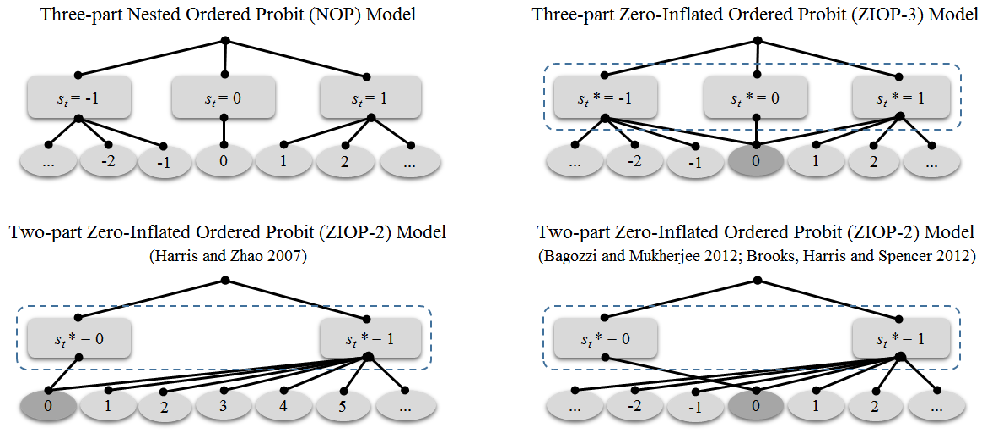
\includegraphics[
natheight=4.0714in, natwidth=9.32in, height=2.8792in, width=6.5529in]
{C:/Users/user/Documents/Dale/Our paper on Github/cnop/paper/graphics/P6UVVI00__1.pdf}%
%EndExpansion
\end{center}

%TCIMACRO{\TeXButton{TeX field}{\justify}}%
%BeginExpansion
\justify%
%EndExpansion
%TCIMACRO{\TeXButton{TeX field}{\footnotesize}}%
%BeginExpansion
\footnotesize%
%EndExpansion

Notes: Decisionmakers are not assumed to choose sequentially. The tree
diagrams simply represent a nesting structure of the system of ordered
probit models.

%TCIMACRO{\TeXButton{E}{\end{figure}}}%
%BeginExpansion
\end{figure}%
%EndExpansion
%TCIMACRO{\TeXButton{Onehalf}{\begin{onehalfspace}}}%
%BeginExpansion
\begin{onehalfspace}%
%EndExpansion

Furthermore, it would be reasonable for the no-change (zero) alternative to
be in three nests: its own one, one with decreases and one with increases;
so some no-change decisions can be driven by similar factors as increases or
decreases. This leads to a three-part cross-nested model with the nests
overlapping at a zero response; hence, the probability of zeros is
`inflated'. Since the regime decision is not observable, the zeros are
observationally equivalent --- it is never known to which of the three nests
the observed zero belongs. While several types of models with overlapping
nests for unordered categorical responses are developed (Vovsha 1997; Wen
and Koppelman 2001), the cross-nested models for ordinal\ outcomes are very
scarce.\footnote{%
Small (1987) introduced an ordered-choice model\ with overlapping nests,
which contain two adjacent choices.}

The prevalence of status quo, neutral or zero outcomes is observed in many
fields, including economics, sociology, technometrics, psychology and
biology. The heterogeneity of zeros is well recognized --- see Winkelmann
(2008) and Greene and Hensher (2010) for a review. Studies discriminate
among different types of zeros such as: no visits to doctor due to good
health, iatrophobia, or medical costs; no children due to infertility or
choice; no illness due to strong resistance or lack of infection. In the
studies of survey responses using an odd-point Likert-type scale, where the
respondents must indicate the negative, neutral or positive attitude or
opinion, the heterogeneity of indifferent responses (a true neutral option
versus an undecided, or ambivalent, or uninformed one, commonly reported as
neutral) is also well-recognized and sometimes labeled as the middle
category endorsement or inflation (Bagozzi and Mukhetjee 2012; Hern\'{a}%
ndez, Drasgow and Gonz\'{a}les-Rom\'{a} 2004; Kulas and Stachowski 2009). In
the decision-making experiments and micro-level studies of consumer choices,
election votes and other repeated choices, the prevalence of no-change
decisions is often attributed to the status quo bias -- a tendency to do
nothing or maintain one's previous decision, even though it is not always
objectively superior to the available options (Hartman, Doane and Woo 1991;
Kahneman, Knetsch, and Thaler 1991). It is a cognitive bias, explained by
both the rational causes (informational or cognitive limitations, transition
or analysis costs) and irrational ones (mental illusions and various
psychological inclinations) --- see Samuelson and Zeckhauser (1988) for an
excellent exposition.

The two-part zero-inflated models, developed to address the unobserved
heterogeneity of zeros, combines a binary choice model for the probability
of crossing the hurdle (to participate or not to participate; to consume or
not to consume) with a count or ordered-choice model for nonnegative
outcomes above the hurdle: the two parts are jointly estimated and the zero
observations can emerge in both parts. The two-part zero-inflated models
include the zero-inflated Poisson (Lambert 1992), negative binomial (Greene
1994), binomial (Hall 2002) and generalized Poisson (Famoye and Singh 2003)
models for count outcomes, and the zero-inflated ordered probit model
(Harris and Zhao 2007) and zero-inflated proportional odds model (Kelley and
Anderson 2008) for non-negative ordinal responses.

The model of Harris and Zhao (2007) is suitable for explaining decisions
such as the levels of consumption, when the upper hurdle is naturally binary
(to smoke or not to smoke) and the ordinal responses are typically
non-negative (see the bottom left panel of Figure \ref{trees}). Thus, the
abundant\ zeros are situated at one end of the ordered scale. Bagozzi and
Mukherjee (2012) and Brooks, Harris and Spencer (2012) extended the model of
Harris and Zhao (2007) and proposed the middle-inflated ordered probit model
for an ordinal outcome, which ranges from negative to positive responses,
and where an abundant outcome is situated in the middle of the choice
spectrum (see the bottom right panel of Figure \ref{trees}).

The three-part cross-nested zero-inflated ordered probit model (see the top
right panel of Figure \ref{trees}), introduced in Sirchenko (2013), is a
natural generalization of the models of Harris and Zhao (2007), Bagozzi and
Mukherjee (2012) and Brooks, Harris and Spencer (2012). A trichotomous
regime decision is more realistic and flexible than a binary decision
(change or no change) if applied to ordinal data with negative, zero and
positive values.

\section{\noindent Models}

\subsection{Notation and assumptions}

The observed dependent variable $y_{t}$, $t=1,2,...,T$ is assumed to take on
a finite number of ordinal values $j$ coded as $%
\{-J^{-},...,-1,0,1,...,J^{+}\},$ where a potentially heterogeneous (and
typically predominant) response is coded as zero. The latent unobserved (or
only partially observed) variables are denoted by $\ast $. Each model
assumes an ordered-choice regime decision and the ordered-choice outcome
decisions conditional on regime. The regime decision is allowed to be
correlated with each outcome decision. We denote by $\mathbf{x}_{t},$ $%
\mathbf{x}_{t}^{-},$ $\mathbf{x}_{t}^{+}$ and $\mathbf{z}_{t}$ the $t^{\text{%
th}}$ rows of the observed data matrices (which in addition to predetermined
explanatory variables may also include the lags of $y_{t}$), by $\mathbf{%
\beta ,}$ $\mathbf{\beta }^{-},$ $\mathbf{\beta }$ and $\mathbf{\gamma }$
the vectors of unknown slope parameters, by $\mathbf{\alpha ,}$ $\mathbf{%
\alpha }^{-}\mathbf{,}$ $\mathbf{\alpha }^{+}$ and $\mathbf{\mu }$ the
vectors of unknown threshold parameters, by $\rho ,$ $\rho ^{-}$ and $\rho
^{+}$ the vectors of unknown correlation coefficients, by $\varepsilon _{t},$
$\varepsilon _{t}^{-},$ $\varepsilon _{t}^{+}$ and $\nu _{t}\ $the error
terms that are independently and identically distributed (\textit{iid})
across $t$ with normal cumulative distribution function (CDF) $\Phi $ and
with variances $\sigma ^{2},$ $\sigma _{-}^{2},$ $\sigma _{+}^{2}$ and $%
\sigma _{\nu }^{2}$, respectively, and by $\Phi _{2}(g_{1}\mathbf{;}g_{2}%
\mathbf{;}\lambda )$ the CDF of the bivariate normal distribution of the two
random variables $g_{1}$ and\textbf{\ }$g_{2}$ with the correlation
coefficient $\rho $ and variances $\sigma _{1}^{2}$ and $\sigma _{2}^{2}$:

\begin{center}
$\Phi _{2}(g_{1}\mathbf{;}g_{2}\mathbf{;}\rho )=\frac{1}{2\pi \sigma
_{1}\sigma _{2}\sqrt{1-\rho ^{2}}}\underset{}{\underset{-\infty }{\overset{%
g_{1}}{\int }}}\underset{-\infty }{\overset{g_{2}}{\int }}\exp \left( -\frac{%
u^{2}/\sigma _{1}^{2}-2\rho uw/\sigma _{1}\sigma _{2}+w^{2}/\sigma _{2}^{2}}{%
2(1-\rho ^{2})}\right) dudw.$
\end{center}

\subsection{Three-part nested ordered probit (NOP) model}

Despite the wide-spread use of nested logit models for unordered categorical
responses we are not aware of any example of the nested ordered probit/logit
model in the literature. The NOP model can be described as

\bigskip

$%
\begin{tabular}{ll}
\ Regime decision: & $r_{t}^{\ast }=\mathbf{z}_{t}\mathbf{\gamma }+\nu _{t},$
\ \ $s_{t}=\left\{ 
\begin{array}{rcl}
1 & \text{if} & \mu _{2}<r_{t}^{\ast }, \\ 
0 & \text{if} & \mu _{1}<r_{t}^{\ast }\leq \mu _{2}, \\ 
-1 & \text{if} & \text{ \ \ \ \ \ \ }r_{t}^{\ast }\leq \mu _{1}.%
\end{array}%
\right. $ \\ 
\ Outcome decisions: & $y_{t}^{-\ast }=\mathbf{x}_{t}^{-}\mathbf{\beta }%
^{-}+\varepsilon _{t}^{-},$ \ \ $y_{t}^{+\ast }=\mathbf{x}_{t}^{+}\mathbf{%
\beta }^{+}+\varepsilon _{t}^{+},$ \\ 
& $y_{t}=\left\{ 
\begin{array}{lcl}
j(j>0) & \text{if} & s_{t}=1\text{ and }\alpha _{j-1}^{+}<y_{t}^{+\ast }\leq
\alpha _{j}^{+}, \\ 
0 & \text{if} & s_{t}=0, \\ 
j(j<0) & \text{if} & s_{t}=-1\text{ \ \ and }\alpha _{j}^{-}<y_{t}^{-\ast
}\leq \alpha _{j+1}^{-},%
\end{array}%
\right. $ \\ 
& where $-\infty =\alpha _{0}^{+}\leq \alpha _{1}^{+}\leq ...\leq \alpha
_{J^{+}}^{+}=\infty $ \\ 
& and $-\infty =\alpha _{-J^{-}}^{-}\leq \alpha _{-J+1}^{-}\leq ...\leq
\alpha _{0}^{-}=\infty $. \\ 
\begin{tabular}{l}
Correlation among \\ 
decisions:%
\end{tabular}
& $\left[ 
\begin{array}{c}
\nu _{t} \\ 
\varepsilon _{t}^{i}%
\end{array}%
\right] \overset{iid}{\sim }\mathcal{N}\left( 
\begin{array}{c}
0 \\ 
0%
\end{array}%
,\left[ 
\begin{array}{cc}
\sigma _{\nu }^{2} & \rho ^{i}\sigma _{\nu }\sigma _{i} \\ 
\rho ^{i}\sigma _{\nu }\sigma _{i} & \sigma _{i}^{2}%
\end{array}%
\right] \right) $, $i\in \{-,+\}.$%
\end{tabular}%
$

\bigskip

The probabilities of the outcome $j$ in the NOP model are given by%
\begin{equation}
\begin{array}{l}
\Pr (y_{t}=j|\mathbf{z}_{t},\mathbf{x}_{t}^{-},\mathbf{x}_{t}^{+})=I_{j<0}%
\Pr (r_{t}^{\ast }\leq \mu _{1}\ \text{and }\alpha _{j}^{-}<y_{t}^{-\ast
}\leq \alpha _{j+1}^{-}|\mathbf{z}_{t},\mathbf{x}_{t}^{-}) \\ 
+I_{j=0}\Pr (\mu _{1}<r_{t}^{\ast }\leq \mu _{2}|\mathbf{z}_{t})+I_{j>0}\Pr
(\mu _{2}<r_{t}^{\ast }\ \text{and }\alpha _{j-1}^{+}<y_{t}^{+\ast }\leq
\alpha _{j}^{+}|\mathbf{z}_{t},\mathbf{x}_{t}^{+}) \\ 
=I_{j<0}\Pr (\nu _{t}\leq \mu _{1}-\mathbf{z}_{t}\mathbf{\gamma }\ \text{and 
}\alpha _{j}^{-}-\mathbf{x}_{t}^{-}\mathbf{\beta }^{-}<\varepsilon
_{t}^{-}\leq \alpha _{j+1}^{-}-\mathbf{x}_{t}^{-}\mathbf{\beta }^{-}) \\ 
+I_{j=0}\Pr (\mu _{1}-\mathbf{z}_{t}\mathbf{\gamma }<\nu _{t}\leq \mu _{2}-%
\mathbf{z}_{t}\mathbf{\gamma }) \\ 
+I_{j>0}\Pr (\mu _{2}-\mathbf{z}_{t}\mathbf{\gamma }<\nu _{t}\ \text{and }%
\alpha _{j-1}^{+}-\mathbf{x}_{t}^{+}\mathbf{\beta }^{+}<\varepsilon
_{t}^{+}\leq \alpha _{j}^{+}-\mathbf{x}_{t}^{+}\mathbf{\beta }^{+}) \\ 
=I_{j<0}[\Phi _{2}(\mu _{1}-\mathbf{z}_{t}\mathbf{\gamma };\alpha _{j+1}^{-}-%
\mathbf{x}_{t}^{-}\mathbf{\beta }^{-}\mathbf{;}\rho ^{-})-\Phi _{2}(\mu _{1}-%
\mathbf{z}_{t}\mathbf{\gamma };\alpha _{j}^{-}-\mathbf{x}_{t}^{-}\mathbf{%
\beta }^{-}\mathbf{;}\rho ^{-})] \\ 
+I_{j=0}[\Phi (\mu _{2}-\mathbf{z}_{t}\mathbf{\gamma })-\Phi (\mu _{1}-%
\mathbf{z}_{t}\mathbf{\gamma })] \\ 
+I_{j>0}[\Phi _{2}(-\mu _{2}+\mathbf{z}_{t}\mathbf{\gamma };\alpha _{j}^{+}-%
\mathbf{x}_{t}^{+}\mathbf{\beta }^{+};\mathbf{-}\rho ^{+})-\Phi _{2}(-\mu
_{2}+\mathbf{z}_{t}\mathbf{\gamma };\alpha _{j-1}^{+}-\mathbf{x}_{t}^{+}%
\mathbf{\beta }^{+};\mathbf{-}\rho ^{+})]\text{,}%
\end{array}
\label{Prob NOP}
\end{equation}

\noindent where $I_{j<0}$ is an indicator function such that $I_{j<0}=1$ if $%
j<0$, and $I_{j<0}=0$ if $j\geq 0$ (analogously for $I_{j=0}$ and $I_{j>0}$).

In the case of exogenous switching (when $\rho ^{-}=\rho ^{+}=0$), the
probabilities of the outcome $j$ in the NOP can be computed as

\begin{center}
$%
\begin{array}{l}
\Pr (y_{t}=j|\mathbf{z}_{t},\mathbf{x}_{t}^{-},\mathbf{x}_{t}^{+},\rho
^{-}=\rho ^{+}=0)=I_{j<0}\Phi (\mu _{1}-\mathbf{z}_{t}\mathbf{\gamma )}[\Phi
(\alpha _{j+1}^{-}-\mathbf{x}_{t}^{-}\mathbf{\beta }^{-})-\Phi (\alpha
_{j}^{-}-\mathbf{x}_{t}^{-}\mathbf{\beta }^{-})] \\ 
+I_{j=0}[\Phi (\mu _{2}-\mathbf{z}_{t}\mathbf{\gamma })-\Phi (\mu _{1}-%
\mathbf{z}_{t}\mathbf{\gamma })] \\ 
+I_{j>0}[1-\Phi (\mu _{2}-\mathbf{z}_{t}\mathbf{\gamma })][\Phi (\alpha
_{j}^{+}-\mathbf{x}_{t}^{+}\mathbf{\beta }^{+})-\Phi (\alpha _{j-1}^{+}-%
\mathbf{x}_{t}^{+}\mathbf{\beta }^{+})]\text{.}%
\end{array}%
$
\end{center}

In the case of three outcome categories the NOP model degenerates to the
conventional single-equation ordered probit model.

\subsection{Two-part zero-inflated ordered probit (ZIOP-2) model}

The ZIOP-2 model, which represents the two part zero-inflated ordered probit
model of Harris and Zhao (2007), Bagozzi and Mukherjee (2012) and Brooks,
Harris and Spencer (2012), can be described by the following system

\medskip

$%
\begin{tabular}{ll}
\ Regime decision: & $r_{t}^{\ast }=\mathbf{z}_{t}\mathbf{\gamma }+\nu _{t},$
\ \ $s_{t}^{\ast }=\left\{ 
\begin{array}{rcl}
1 & \text{if} & \mu <r_{t}^{\ast }, \\ 
0 & \text{if} & r_{t}^{\ast }\leq \mu .%
\end{array}%
\right. $ \\ 
\ Outcome decision: \ \ \ \ \ \  & $y_{t}^{\ast }=\mathbf{x}_{t}\mathbf{%
\beta }+\varepsilon _{t},$ \\ 
& $y_{t}=\left\{ 
\begin{array}{lcl}
j & \text{if} & s_{t}^{\ast }=1\text{ and }\alpha _{j-1}<y_{t}^{\ast }\leq
\alpha _{j}, \\ 
0 & \text{if} & s_{t}^{\ast }=0,%
\end{array}%
\right. $ \\ 
& where $-\infty =\alpha _{-J^{-}-1}\leq \alpha _{-J^{-}}\leq ...\leq \alpha
_{J^{+}}=\infty .$ \\ 
\begin{tabular}{l}
Correlation among \\ 
decisions:%
\end{tabular}
& $\left[ 
\begin{array}{c}
\nu _{t} \\ 
\varepsilon _{t}%
\end{array}%
\right] \overset{iid}{\sim }\mathcal{N}\left( 
\begin{array}{c}
0 \\ 
0%
\end{array}%
,\left[ 
\begin{array}{cc}
\sigma _{\nu }^{2} & \rho \sigma _{\nu }\sigma _{\varepsilon } \\ 
\rho \sigma _{\nu }\sigma _{\varepsilon } & \sigma _{\varepsilon }^{2}%
\end{array}%
\right] \right) .$%
\end{tabular}%
$

\bigskip

The probabilities of the outcome $j$ in the ZIOP-2 model are given by%
\begin{equation}
\begin{array}{l}
\Pr (y_{t}=j|\mathbf{z}_{t},\mathbf{x}_{t})=I_{j=0}\Pr (r_{t}^{\ast }\leq
\mu |\mathbf{z}_{t})+I_{j\geq 0}\Pr (\mu <r_{t}^{\ast }\ \text{and }\alpha
_{j-1}<y_{t}^{\ast }\leq \alpha _{j}|\mathbf{z}_{t},\mathbf{x}_{t}) \\ 
=I_{j=0}\Pr (\nu _{t}\leq \mu -\mathbf{z}_{t}\mathbf{\gamma })+I_{j\geq
0}\Pr (\mu -\mathbf{z}_{t}\mathbf{\gamma }<\nu _{t}\ \text{and }\alpha
_{j-1}-\mathbf{x}_{t}\mathbf{\beta }<\varepsilon _{t}\leq \alpha _{j}-%
\mathbf{x}_{t}\mathbf{\beta }) \\ 
=I_{j=0}\Phi (\mu -\mathbf{z}_{t}\mathbf{\gamma })+\Phi _{2}(-\mu +\mathbf{z}%
_{t}\mathbf{\gamma };\alpha _{j}-\mathbf{x}_{t}\mathbf{\beta };\mathbf{-}%
\rho )-\Phi _{2}(-\mu +\mathbf{z}_{t}\mathbf{\gamma };\alpha _{j-1}-\mathbf{x%
}_{t}\mathbf{\beta };\mathbf{-}\rho )\text{.}%
\end{array}
\label{Prob MIOP}
\end{equation}

In the case of exogenous switching (when $\rho =0$), the probabilities of
the outcome $j$ in the ZIOP-2 model can be computed as

\begin{center}
$\Pr (y_{t}=j|\mathbf{z}_{t},\mathbf{x}_{t},\rho =0)=I_{j=0}\Phi (\mu -%
\mathbf{z}_{t}\mathbf{\gamma })+[1-\Phi (\mu -\mathbf{z}_{t}\mathbf{\gamma }%
)][\Phi (\alpha _{j}-\mathbf{x}_{t}\mathbf{\beta })-\Phi (\alpha _{j-1}-%
\mathbf{x}_{t}\mathbf{\beta })]$.
\end{center}

If $y_{t}\geq 0$ for $\forall t,$ the ZIOP-2 model represents the model of
Harris and Zhao (2007).

\subsection{Three-part zero-inflated ordered probit (ZIOP-3) model}

The ZIOP-3 model, developed by Sirchenko (2013), is a three-part
generalization of the ZIOP-2 model, and can be described by the following
system

\medskip

$%
\begin{tabular}{ll}
\ Regime decision: & $r_{t}^{\ast }=\mathbf{z}_{t}\mathbf{\gamma }+\nu _{t},$
\ \ $s_{t}^{\ast }=\left\{ 
\begin{array}{rcl}
1 & \text{if} & \mu _{2}<r_{t}^{\ast }, \\ 
0 & \text{if} & \mu _{1}<r_{t}^{\ast }\leq \mu _{2}, \\ 
-1 & \text{if} & \text{ \ \ \ \ \ \ }r_{t}^{\ast }\leq \mu _{1}.%
\end{array}%
\right. $ \\ 
\ Outcome decisions: & $y_{t}^{-\ast }=\mathbf{x}_{t}^{-}\mathbf{\beta }%
^{-}+\varepsilon _{t}^{-},$ \ \ $y_{t}^{+\ast }=\mathbf{x}_{t}^{+}\mathbf{%
\beta }^{+}+\varepsilon _{t}^{+},$ \\ 
& $y_{t}=\left\{ 
\begin{array}{lcl}
j(j\geq 0) & \text{if} & s_{t}^{\ast }=1\text{ \ \ and }\alpha
_{j-1}^{+}<y_{t}^{+\ast }\leq \alpha _{j}^{+}, \\ 
0 & \text{if} & s_{t}^{\ast }=0, \\ 
j(j\leq 0) & \text{if} & s_{t}^{\ast }=-1\text{ and }\alpha
_{j}^{-}<y_{t}^{-\ast }\leq \alpha _{j+1}^{-},%
\end{array}%
\right. $ \\ 
& where $-\infty =\alpha _{-1}^{+}\leq \alpha _{0}^{+}\leq ...\leq \alpha
_{J^{+}}^{+}=\infty $ \\ 
& and $-\infty =\alpha _{-J^{-}}^{-}\leq \alpha _{-J+1}^{-}\leq ...\leq
\alpha _{1}^{-}=\infty $. \\ 
\begin{tabular}{l}
Correlation among \\ 
decisions:%
\end{tabular}
& $\left[ 
\begin{array}{c}
\nu _{t} \\ 
\varepsilon _{t}^{i}%
\end{array}%
\right] \overset{iid}{\sim }\mathcal{N}\left( 
\begin{array}{c}
0 \\ 
0%
\end{array}%
,\left[ 
\begin{array}{cc}
\sigma _{\nu }^{2} & \rho ^{i}\sigma _{\nu }\sigma _{i} \\ 
\rho ^{i}\sigma _{\nu }\sigma _{i} & \sigma _{i}^{2}%
\end{array}%
\right] \right) $, $i\in \{-,+\}.$%
\end{tabular}%
$

\bigskip

The probabilities of the outcome $j$ in the ZIOP-3 model are given by

\begin{flushleft}
\begin{equation}
\begin{array}{l}
\Pr (y_{t}=j|\mathbf{z}_{t},\mathbf{x}_{t}^{-},\mathbf{x}_{t}^{+})=I_{j\leq
0}\Pr (r_{t}^{\ast }\leq \mu _{1}\ \text{and }\alpha _{j}^{-}<y_{t}^{-\ast
}\leq \alpha _{j+1}^{-}|\mathbf{z}_{t},\mathbf{x}_{t}^{-}) \\ 
+I_{j=0}\Pr (\mu _{1}<r_{t}^{\ast }\leq \mu _{2}|\mathbf{z}_{t})+I_{j\geq
0}\Pr (\mu _{2}<r_{t}^{\ast }\ \text{and }\alpha _{j-1}^{+}<y_{t}^{+\ast
}\leq \alpha _{j}^{+}|\mathbf{z}_{t},\mathbf{x}_{t}^{+}) \\ 
=I_{j\leq 0}\Pr (\nu _{t}\leq \mu _{1}-\mathbf{z}_{t}\mathbf{\gamma }\ \text{%
and }\alpha _{j}^{-}-\mathbf{x}_{t}^{-}\mathbf{\beta }^{-}<\varepsilon
_{t}^{-}\leq \alpha _{j+1}^{-}-\mathbf{x}_{t}^{-}\mathbf{\beta }^{-}) \\ 
+I_{j=0}\Pr (\mu _{1}-\mathbf{z}_{t}\mathbf{\gamma }<\nu _{t}\leq \mu _{2}-%
\mathbf{z}_{t}\mathbf{\gamma }) \\ 
+I_{j\geq 0}\Pr (\mu _{2}-\mathbf{z}_{t}\mathbf{\gamma }<\nu _{t}\ \text{and 
}\alpha _{j-1}^{+}-\mathbf{x}_{t}^{+}\mathbf{\beta }^{+}<\varepsilon
_{t}^{+}\leq \alpha _{j}^{+}-\mathbf{x}_{t}^{+}\mathbf{\beta }^{+}) \\ 
=I_{j\leq 0}[\Phi _{2}(\mu _{1}-\mathbf{z}_{t}\mathbf{\gamma };\alpha
_{j+1}^{-}-\mathbf{x}_{t}^{-}\mathbf{\beta }^{-}\mathbf{;}\rho ^{-})-\Phi
_{2}(\mu _{1}-\mathbf{z}_{t}\mathbf{\gamma };\alpha _{j}^{-}-\mathbf{x}%
_{t}^{-}\mathbf{\beta }^{-}\mathbf{;}\rho ^{-})] \\ 
+I_{j=0}[\Phi (\mu _{2}-\mathbf{z}_{t}\mathbf{\gamma })-\Phi (\mu _{1}-%
\mathbf{z}_{t}\mathbf{\gamma })] \\ 
+I_{j\geq 0}[\Phi _{2}(-\mu _{2}+\mathbf{z}_{t}\mathbf{\gamma };\alpha
_{j}^{+}-\mathbf{x}_{t}^{+}\mathbf{\beta }^{+};\mathbf{-}\rho ^{+})-\Phi
_{2}(-\mu _{2}+\mathbf{z}_{t}\mathbf{\gamma };\alpha _{j-1}^{+}-\mathbf{x}%
_{t}^{+}\mathbf{\beta }^{+};\mathbf{-}\rho ^{+})]\text{,}%
\end{array}
\label{Prob CroNOP}
\end{equation}
\end{flushleft}

\noindent where $I_{j\leq 0}$ is an indicator function such that $I_{j\leq
0}=1$ if $j\leq 0$, and $I_{j\leq 0}=0$ if $j>0$ (analogously for $I_{j\geq
0}$).

In the case of exogenous switching (when $\rho ^{-}=\rho ^{+}=0$), the
probabilities of the outcome $j$ in the ZIOP-3 model can be computed as

\begin{center}
$%
\begin{array}{l}
\Pr (y_{t}=j|\mathbf{z}_{t},\mathbf{x}_{t}^{-},\mathbf{x}_{t}^{+},\rho
^{-}=\rho ^{+}=0)=I_{j\leq 0}\Phi (\mu _{1}-\mathbf{z}_{t}\mathbf{\gamma )}%
[\Phi (\alpha _{j+1}^{-}-\mathbf{x}_{t}^{-}\mathbf{\beta }^{-})-\Phi (\alpha
_{j}^{-}-\mathbf{x}_{t}^{-}\mathbf{\beta }^{-})] \\ 
+I_{j=0}[\Phi (\mu _{2}-\mathbf{z}_{t}\mathbf{\gamma })-\Phi (\mu _{1}-%
\mathbf{z}_{t}\mathbf{\gamma })] \\ 
+I_{j\geq 0}[1-\Phi (\mu _{2}-\mathbf{z}_{t}\mathbf{\gamma })][\Phi (\alpha
_{j}^{+}-\mathbf{x}_{t}^{+}\mathbf{\beta }^{+})-\Phi (\alpha _{j-1}^{+}-%
\mathbf{x}_{t}^{+}\mathbf{\beta }^{+})]\text{.}%
\end{array}%
$
\end{center}

The inflated outcome does not have to be in the \emph{very} middle of
ordered categories. If it is located at the \emph{end} of the ordered scale,
i.e. if $y_{t}\geq 0$ for $\forall t,$ the ZIOP-3 model reduces to the
ZIOP-2 model of Harris and Zhao (2007).

\subsection{Maximum likelihood (ML) estimation}

The probabilities in each ordered probit model representing the regime and
outcome decisions can be consistently estimated under fairly general
conditions by an asymptotically normal ML estimator (Basu and de Jong 2007).
The simultaneous estimation of the ordered probit equations in the NOP,
ZIOP-2 and ZIOP-3 models can be performed using an ML estimator of the
vector of the parameters $\mathbf{\theta }$ that solves

\begin{equation}
\underset{\mathbf{\theta \epsilon \Theta }}{\max }\overset{}{\underset{}{%
\underset{t=1}{\overset{T}{\sum }}}}\overset{J^{+}}{\underset{j=-J^{-}}{\sum 
}}I_{tj}\ln [\Pr (y_{t}=j|\mathbf{x}_{t}^{all},\mathbf{\theta })]\text{,}
\label{LL}
\end{equation}

\noindent where $I_{tj}$ is an indicator function such that $I_{tj}=1$ if $%
y_{t}=j$ and $I_{tj}=0$ otherwise; $\mathbf{\theta }$ includes: $\mathbf{%
\gamma ,}$ $\mathbf{\mu ,}$ $\mathbf{\beta }^{-},$ $\mathbf{\beta }^{+},$ $%
\mathbf{\alpha }^{-}$ and $\mathbf{\alpha }^{+}$ (for the NOP model), $%
\mathbf{\gamma },$ $\mu ,$ $\mathbf{\beta },$ $\mathbf{\alpha }$ and $\rho $
(for the ZIOP-2 model) and $\mathbf{\gamma },$ $\mathbf{\mu },$ $\mathbf{%
\beta }^{-},$ $\mathbf{\beta }^{+},$ $\mathbf{\alpha }^{-},$ $\mathbf{\alpha 
}^{+},$ $\rho ^{-}$ and $\rho ^{+}$ (for the ZIOP-3 model); $\Theta $ is a
parameters' space; $\mathbf{x}_{t}^{all}$ is a vector that contains the
values of all covariates in the model; and $\Pr (y_{t}=j|\mathbf{x}%
_{t}^{all},\mathbf{\theta })$ are probabilities in either (\ref{Prob NOP})
or (\ref{Prob MIOP}) or (\ref{Prob CroNOP}) for, respectively, the NOP,
ZIOP-2 and ZIOP-3 models. The asymptotic standard errors of $\widehat{%
\mathbf{\theta }}$ can be computed from the Hessian matrix.

The intercept components of $\mathbf{\beta ,}$ $\mathbf{\beta }^{-},$ $%
\mathbf{\beta }$ and $\mathbf{\gamma }$ are identified up to scale and
location, that is only jointly with the corresponding threshold parameters $%
\mathbf{\alpha ,}$ $\mathbf{\alpha }^{-}\mathbf{,}$ $\mathbf{\alpha }^{+}$
and $\mathbf{\mu }$ and variances $\sigma ^{2},$ $\sigma _{-}^{2},$ $\sigma
_{+}^{2},$ and $\sigma _{\nu }^{2}$. As is common in the identification of
discrete choice models, the variances $\sigma ^{2},$ $\sigma _{-}^{2},$ $%
\sigma _{+}^{2},$ and $\sigma _{\nu }^{2}$ are fixed to one, and the
intercept components of $\mathbf{\beta ,}$ $\mathbf{\beta }^{-},$ $\mathbf{%
\beta }$ and $\mathbf{\gamma }$ are fixed to zero. The probabilities are
invariant to these (arbitrary) identifying assumptions: up to scale and
location, we can identify all parameters in $\mathbf{\theta }$ because of
the nonlinearity of ordered probit equations, i.e. via the functional form
(Heckman 1978; Wilde 2000). However, since the normal CDF is approximately
linear in the middle of its support, the simultaneous estimation of two or
three equations may experience a weak identification problem if regime and
outcome equations contain the same set of covariates. To enhance the
precision of parameter estimates we may impose exclusion restrictions on the
specification of covariates in each equation.

The three regimes (nests) in the NOP model are fully observable, contrary to
the latent (only partially observed) regimes in the ZIOP-2 and ZIOP-3
models. The likelihood function of the NOP model ---\ again in contrast with
the ZIOP-2 and ZIOP-3 models --- is separable with respect to the parameters
in the three equations. Thus, solving (\ref{LL}) for the NOP model is
equivalent to maximizing separately the likelihoods of the three ordered
probit models representing the regime and outcome decisions.\footnote{%
The data matrices in the outcome decisions should be truncated to contain
only those rows of $\mathbf{x}_{t}^{-}$ or $\mathbf{x}_{t}^{+}$ for which $%
y_{t}<0$ or $y_{t}>0$, respectively.}

\subsection{Marginal effects (ME)}

\noindent The marginal effect of a continuous covariate $k$ (the $k^{\text{th%
}}$ element of $\mathbf{x}_{t}^{all}$) on the probability of each discrete
outcome $j$ are computed for the ZIOP-3 model as

\bigskip

$%
\begin{array}{l}
ME_{k,j,t}=\frac{\partial \Pr (y_{t}=j|\mathbf{\theta })}{\partial \mathbf{x}%
_{t,k}^{all}}=I_{j\leq 0}\left\{ \left[ \Phi \left( \frac{\mu _{1}-\mathbf{z}%
_{t}\mathbf{\gamma }-\rho ^{-}(\alpha _{j}^{-}-\mathbf{x}_{t}^{-}\mathbf{%
\beta ^{-})}}{\sqrt{1-(\rho ^{-})^{2}}}\right) f(\alpha _{j}^{-}-\mathbf{x}%
_{t}^{-}\mathbf{\beta ^{-}})\right. \right. \\ 
\left. -\Phi \left( \frac{\mu _{1}-\mathbf{z}_{t}\mathbf{\gamma }-\rho
^{-}(\alpha _{j+1}^{-}-\mathbf{x}_{t}^{-}\mathbf{\beta ^{-})}}{\sqrt{1-(\rho
^{-})^{2}}}\right) f(\alpha _{j+1}^{-}-\mathbf{x}_{t}^{-}\mathbf{\beta ^{-}})%
\right] \mathbf{\beta }_{k}^{-all} \\ 
\left. -\left[ \Phi \left( \frac{\alpha _{j+1}^{-}-\mathbf{x}_{t}^{-}\mathbf{%
\beta ^{-}}-\rho ^{-}(\mu _{1}-\mathbf{z}_{t}\mathbf{\gamma )}}{\sqrt{%
1-(\rho ^{-})^{2}}}\right) -\Phi \left( \frac{\alpha _{j}^{-}-\mathbf{x}%
_{t}^{-}\mathbf{\beta ^{-}}-\rho ^{-}(\mu _{1}-\mathbf{z}_{t}\mathbf{\gamma )%
}}{\sqrt{1-(\rho ^{-})^{2}}}\right) \right] f(\mu _{1}-\mathbf{z}_{t}\mathbf{%
\gamma })\mathbf{\gamma }_{k}^{all}\right\} \\ 
-I_{j=0}[f(\mu _{2}-\mathbf{z}_{t}\mathbf{\gamma })-f(\mu _{1}-\mathbf{z}_{t}%
\mathbf{\gamma })]\mathbf{\gamma }_{k}^{all} \\ 
+I_{j\geq 0}\left\{ \left[ \Phi \left( \frac{\mathbf{z}_{t}\mathbf{\gamma }%
-\mu _{2}+\rho ^{+}(\alpha _{j-1}^{+}-\mathbf{x}_{t}^{+}\mathbf{\beta ^{+})}%
}{\sqrt{1-(\rho ^{+})^{2}}}\right) \right. \right. f(\alpha _{j-1}^{+}-%
\mathbf{x}_{t}^{+}\mathbf{\beta ^{+}}) \\ 
\left. -\Phi \left( \frac{\mathbf{z}_{t}\mathbf{\gamma }-\mu _{2}+\rho
^{+}(\alpha _{j}^{+}-\mathbf{x}_{t}^{+}\mathbf{\beta ^{+})}}{\sqrt{1-(\rho
^{+})^{2}}}\right) f(\alpha _{j}^{+}-\mathbf{x}_{t}^{+}\mathbf{\beta ^{+}})%
\right] \mathbf{\beta }_{k}^{+all} \\ 
\left. +\left[ \Phi \left( \frac{\alpha _{j}^{+}-\mathbf{x}_{t}^{+}\mathbf{%
\beta ^{+}}+\rho ^{+}(\mathbf{z}_{t}\mathbf{\gamma }-\mu _{2}\mathbf{)}}{%
\sqrt{1-(\rho ^{+})^{2}}}\right) -\Phi \left( \frac{\alpha _{j-1}^{+}-%
\mathbf{x}_{t}^{+}\mathbf{\beta ^{+}}+\rho ^{+}(\mathbf{z}_{t}\mathbf{\gamma 
}-\mu _{2}\mathbf{)}}{\sqrt{1-(\rho ^{+})^{2}}}\right) \right] f(\mathbf{z}%
_{t}\mathbf{\gamma }-\mu _{2})\mathbf{\gamma }_{k}^{all}\right\} ,%
\end{array}%
$

\bigskip

\noindent where $f$ is the probability density function of the standard
normal distribution, and $\mathbf{\gamma }_{k}^{all}$, $\mathbf{\beta }%
_{k}^{-all}$ and $\mathbf{\beta }_{k}^{+all}$ are the coefficients on the $%
k^{\text{th}}$ covariate in $\mathbf{x}_{t}^{all}$ in the regime equation,
outcome equation conditional on $s_{t}^{\ast }=1$ and outcome equation
conditional on $s_{t}^{\ast }=-1$, respectively ($\mathbf{\gamma }_{k}^{all}$%
, $\mathbf{\beta }_{k}^{-all}$ or $\mathbf{\beta }_{k}^{+all}$ is zero if
the $k^{\text{th}}$ covariate in $\mathbf{x}_{t}^{all}$ is not included into
the corresponding equation). For a discrete-valued covariate, the ME can be
computed as the change in the probabilities when this covariate changes by
one increment and all other covariates are fixed.

The MEs for the NOP model are computed by replacing $I_{j\geq 0}$ with $%
I_{j>0}$ and $I_{j\leq 0}$ with $I_{j<0}$. The MEs for the ZIOP-2 model are
computed as

\bigskip

$%
\begin{array}{l}
ME_{k,j,t}=\frac{\partial \Pr (y_{t}=j|\mathbf{\theta })}{\partial \mathbf{x}%
_{t,k}^{all}}=-I_{j=0}[f(\mu -\mathbf{z}_{t}\mathbf{\gamma })]\mathbf{\gamma 
}_{k}^{all} \\ 
+\left[ \Phi \left( \frac{\mathbf{z}_{t}\mathbf{\gamma }-\mu +\rho (\alpha
_{j-1}-\mathbf{x}_{t}\mathbf{\beta )}}{\sqrt{1-\rho ^{2}}}\right) f(\alpha
_{j-1}-\mathbf{x}_{t}\mathbf{\beta })-\Phi \left( \frac{\mathbf{z}_{t}%
\mathbf{\gamma }-\mu +\rho (\alpha _{j}-\mathbf{x}_{t}\mathbf{\beta )}}{%
\sqrt{1-\rho ^{2}}}\right) f(\alpha _{j}-\mathbf{x}_{t}\mathbf{\beta })%
\right] \mathbf{\beta }_{k}^{all} \\ 
+\left[ \Phi \left( \frac{\alpha _{j}-\mathbf{x}_{t}\mathbf{\beta }+\rho (%
\mathbf{z}_{t}\mathbf{\gamma }-\mu \mathbf{)}}{\sqrt{1-\rho ^{2}}}\right)
-\Phi \left( \frac{\alpha _{j-1}-\mathbf{x}_{t}\mathbf{\beta }+\rho (\mathbf{%
z}_{t}\mathbf{\gamma }-\mu \mathbf{)}}{\sqrt{1-\rho ^{2}}}\right) \right] f(%
\mathbf{z}_{t}\mathbf{\gamma }-\mu )\mathbf{\gamma }_{k}^{all}\text{,}%
\end{array}%
$

\bigskip

\noindent where $\mathbf{\beta }_{k}^{all}$ is the coefficient on the $k^{%
\text{th}}$ covariate in $\mathbf{x}_{t}^{all}$ in the outcome equation ($%
\mathbf{\beta }_{k}^{all}$ is zero if the $k^{\text{th}}$ covariate in $%
\mathbf{x}_{t}^{all}$ is not included into the outcome equation).

The asymptotic standard errors of the MEs are computed using the Delta
method as the square roots of the diagonal elements of

\begin{center}
$\widehat{Var(\widehat{\underset{}{\mathbf{ME}_{k,j,t}}})}=\nabla _{\theta }%
\widehat{\mathbf{ME}}_{k,j,t}\widehat{Var(\widehat{\mathbf{\theta }})}\nabla
_{\theta }\widehat{\mathbf{ME}}_{k,j,t})^{\prime }$.
\end{center}

\subsection{\noindent Relations among the models and their comparison}

The choice of a formal model-selection test depends on whether the models
are nested in each other.

The exogenous-switching version of each model is nested in its
endogenous-switching version as its uncorrelated special case; their
comparison can be performed using any classical lilkelihood-based test for
nested hypotheses, such as the likelihood ratio (LR) test.

The NOP model is nested in the ZIOP-3 model. The latter becomes a NOP model
if $\alpha _{-1}^{-}\rightarrow \infty $ and $\alpha _{1}^{+}\rightarrow
-\infty $; therefore, $\Pr (y_{t}=0|\mathbf{x}_{t}^{+},s_{t}=1)\rightarrow 0$
and $\Pr (y_{t}=0|\mathbf{x}_{t}^{-},s_{t}=-1)\rightarrow 0$. Thus, the
comparison of the NOP and ZIOP-3 models can also be performed with the LR
test; however, the critical values of the classical LR test are invalid
since some standard regularity conditions of the classical LR test fail to
hold. In particular, the values of $\alpha _{-1}^{-}$ and $\alpha _{1}^{+}$
in the null hypothesis are not the interior points of the parameter space;
hence, the asymptotic distribution of the LR statistics is not standard.
Instead, we may use the simulated critical values provided in Andrews (2001).

Generally, the ZIOP-2 model is not a special case of the ZIOP-3 model, and
vice versa. However, they are not strictly non-nested and overlap if all
their slope parameters are fixed to zeros. We can compare them using a
likelihood-based test for non-nested overlapping models, such as the Vuong
test (Vuong 1989). A special case when the ZIOP-3 model nests the ZIOP-2
model emerges under some restrictions on the parameters as explained below.
In this case, the selection between the ZIOP-3 and ZIOP-2 models can be
performed using any classical likelihood-based test for nested hypotheses,
which can be interpreted as a misspecification test for the latter.

The special case emerges if $y_{t}$ takes only three discrete choices $j\in
\{-1,0,1\}$, the regressors in $\mathbf{x}_{t}^{-}$ and $\mathbf{x}_{t}^{+}$
in the outcome equations of the ZIOP-3 model contain all regressors (denoted
below by $\mathbf{z}_{2t}$ with the parameter vector $\mathbf{\gamma }_{2}$)
in the ZIOP-2 regime equation, and the regressors (denoted below by $\mathbf{%
z}_{3t}$ with the parameter vector $\mathbf{\gamma }_{3}$) in the regime
equation of the ZIOP-3 model include all regressors in the $\mathbf{x}_{t}$
in the ZIOP-2 outcome equation. According to\ (\ref{Prob MIOP}) the
probabilities of the outcome $j$ in the ZIOP-2 model are given by

\begin{flushleft}
\begin{equation}
\begin{array}{l}
\Pr (y_{t}=-1|\mathbf{z}_{2t},\mathbf{x}_{t})=\Phi _{2}(-\mu +\mathbf{z}_{2t}%
\mathbf{\gamma }_{2};\alpha _{-1}-\mathbf{x}_{t}\mathbf{\beta };\mathbf{-}%
\rho ); \\ 
\Pr (y_{t}=0|\mathbf{z}_{2t},\mathbf{x}_{t})=\Phi (\mu -\mathbf{z}_{2t}%
\mathbf{\gamma }_{2}) \\ 
+\Phi _{2}(-\mu +\mathbf{z}_{2t}\mathbf{\gamma }_{2};\alpha _{0}-\mathbf{x}%
_{t}\mathbf{\beta };\mathbf{-}\rho )-\Phi _{2}(-\mu +\mathbf{z}_{2t}\mathbf{%
\gamma }_{2};\alpha _{-1}-\mathbf{x}_{t}\mathbf{\beta };\mathbf{-}\rho ) \\ 
=1-\Phi _{2}(-\mu +\mathbf{z}_{2t}\mathbf{\gamma }_{2};-\alpha _{0}+\mathbf{x%
}_{t}\mathbf{\beta };\rho )-\Phi _{2}(-\mu +\mathbf{z}_{2t}\mathbf{\gamma }%
_{2};\alpha _{-1}-\mathbf{x}_{t}\mathbf{\beta };\mathbf{-}\rho ); \\ 
\Pr (y_{t}=1|\mathbf{z}_{2t},\mathbf{x}_{t})=\Phi (-\mu +\mathbf{z}_{2t}%
\mathbf{\gamma })-\Phi _{2}(-\mu +\mathbf{z}_{2t}\mathbf{\gamma }_{2};\alpha
_{0}-\mathbf{x}_{t}\mathbf{\beta };\mathbf{-}\rho ) \\ 
=\Phi _{2}(-\mu +\mathbf{z}_{2t}\mathbf{\gamma }_{2};-\alpha _{0}+\mathbf{x}%
_{t}\mathbf{\beta };\rho ),%
\end{array}
\label{Prob spec ZIOP-2}
\end{equation}
\end{flushleft}

\noindent since $\Phi _{2}(x;y;\rho )=\Phi (x)-\Phi _{2}(x;-y;-\rho )$.
Similarly, according to (\ref{Prob CroNOP}) the probabilities of the outcome 
$j$ in the ZIOP-3 model are given by

\begin{flushleft}
\begin{equation}
\begin{array}{l}
\Pr (y_{t}=-1|\mathbf{z}_{3t},\mathbf{x}_{t}^{-},\mathbf{x}_{t}^{+})=\Phi
_{2}(\mu _{1}-\mathbf{z}_{3t}\mathbf{\gamma }_{3};\alpha _{0}^{-}-\mathbf{x}%
_{t}^{-}\mathbf{\beta }^{-}\mathbf{;}\rho ^{-}); \\ 
\Pr (y_{t}=0|\mathbf{z}_{3t},\mathbf{x}_{t}^{-},\mathbf{x}_{t}^{+})=\Phi
(\mu _{1}-\mathbf{z}_{3t}\mathbf{\gamma }_{3})-\Phi _{2}(\mu _{1}-\mathbf{z}%
_{3t}\mathbf{\gamma }_{3};\alpha _{0}^{-}-\mathbf{x}_{t}^{-}\mathbf{\beta }%
^{-}\mathbf{;}\rho ^{-}) \\ 
+\Phi (\mu _{2}-\mathbf{z}_{3t}\mathbf{\gamma }_{3})-\Phi (\mu _{1}-\mathbf{z%
}_{3t}\mathbf{\gamma }_{3})+\Phi _{2}(-\mu _{2}+\mathbf{z}_{3t}\mathbf{%
\gamma }_{3};\alpha _{0}^{+}-\mathbf{x}_{t}^{+}\mathbf{\beta }^{+};\mathbf{-}%
\rho ^{+}) \\ 
=\Phi _{2}(\mu _{1}-\mathbf{z}_{3t}\mathbf{\gamma }_{3};-\alpha _{0}^{-}+%
\mathbf{x}_{t}^{-}\mathbf{\beta }^{-}\mathbf{;-}\rho ^{-}) \\ 
+\Phi (\mu _{2}-\mathbf{z}_{3t}\mathbf{\gamma }_{3})-\Phi (\mu _{1}-\mathbf{z%
}_{3t}\mathbf{\gamma }_{3})+\Phi _{2}(-\mu _{2}+\mathbf{z}_{3t}\mathbf{%
\gamma }_{3};\alpha _{0}^{+}-\mathbf{x}_{t}^{+}\mathbf{\beta }^{+};\mathbf{-}%
\rho ^{+}); \\ 
\Pr (y_{t}=1|\mathbf{z}_{3t},\mathbf{x}_{t}^{-},\mathbf{x}_{t}^{+})=\Phi
(-\mu _{2}+\mathbf{z}_{3t}\mathbf{\gamma }_{3})-\Phi _{2}(-\mu _{2}+\mathbf{z%
}_{3t}\mathbf{\gamma }_{3};\alpha _{0}^{+}-\mathbf{x}_{t}^{+}\mathbf{\beta }%
^{+};\mathbf{-}\rho ^{+}) \\ 
=\Phi _{2}(-\mu _{2}+\mathbf{z}_{3t}\mathbf{\gamma }_{3};-\alpha _{0}^{+}+%
\mathbf{x}_{t}^{+}\mathbf{\beta }^{+};\rho ^{+}).%
\end{array}
\label{Prob spec ZIOP-3}
\end{equation}
\end{flushleft}

Suppose the covariates in $\mathbf{x}_{t}^{-}$ and $\mathbf{x}_{t}^{+}$ in
the ZIOP-3 outcome equations are identical to the covariates in $\mathbf{z}%
_{t}^{2}$ in the ZIOP-2 regime equation, the covariates in $\mathbf{z}_{3t}$
in the ZIOP-3 regime equation are identical to the covariates in the $%
\mathbf{x}_{t}$ in the ZIOP-2 outcome equation, and the parameters are
restricted as follows: $-\mathbf{\beta }^{-}=\mathbf{\beta }^{+}=\mathbf{%
\gamma }_{2},$ $\mathbf{\beta }=\mathbf{\gamma }_{3},$ $\mu _{1}=\alpha
_{-1},$ $\mu _{2}=\alpha _{0},$ $-\alpha _{0}^{-}=\alpha _{0}^{+}=\mu $ and $%
-\rho ^{-}=\rho ^{+}=\rho $. Then, since $\mathbf{x}_{t}^{-}=\mathbf{x}%
_{t}^{+}=\mathbf{z}_{2t}$, $\mathbf{z}_{3t}=\mathbf{x}_{t}$ and $\Phi
(-x)=1-\Phi (x)$, the probabilities for the ZIOP-3 model in (\ref{Prob spec
ZIOP-3}) can be written as

\bigskip

$%
\begin{array}{l}
\Pr (y_{t}=-1|\mathbf{x}_{t},\mathbf{z}_{2t})=\Phi _{2}(\alpha _{-1}-\mathbf{%
x}_{t}\mathbf{\beta };-\mu +\mathbf{z}_{2t}\mathbf{\gamma }_{2}\mathbf{;-}%
\rho ); \\ 
\Pr (y_{t}=0|\mathbf{x}_{t},\mathbf{z}_{2t})=\Phi _{2}(\alpha _{-1}-\mathbf{x%
}_{t}\mathbf{\beta };\mu -\mathbf{z}_{2t}\mathbf{\gamma }_{2}\mathbf{;}\rho )
\\ 
+\Phi (\alpha _{0}-\mathbf{x}_{t}\mathbf{\beta })-\Phi (\alpha _{-1}-\mathbf{%
x}_{t}\mathbf{\beta })+\Phi _{2}(-\alpha _{0}+\mathbf{x}_{t}\mathbf{\beta }%
;\mu -\mathbf{z}_{2t}\mathbf{\gamma }_{2};\mathbf{-}\rho ) \\ 
=-\Phi _{2}(\alpha _{-1}-\mathbf{x}_{t}\mathbf{\beta };-\mu +\mathbf{z}_{2t}%
\mathbf{\gamma }_{2}\mathbf{;-}\rho )+1-\Phi _{2}(-\alpha _{0}+\mathbf{x}_{t}%
\mathbf{\beta };-\mu +\mathbf{z}_{2t}\mathbf{\gamma }_{2};\rho ); \\ 
\Pr (y_{t}=1|\mathbf{x}_{t},\mathbf{z}_{2t})=\Phi _{2}(-\alpha _{0}+\mathbf{x%
}_{t}\mathbf{\beta };-\mu +\mathbf{z}_{2t}\mathbf{\gamma }_{2};\rho ),%
\end{array}%
$

\bigskip

\noindent which are identical to the probabilities for the ZIOP-2 model in (%
\ref{Prob spec ZIOP-2}). Notice that the restrictions $-\mathbf{\beta }^{-}=%
\mathbf{\beta }^{+}=\mathbf{\gamma }_{2}$ and $-\alpha _{0}^{-}=\alpha
_{0}^{+}=\mu $ impose a sort of symmetry in the ZIOP-3 model because they
imply that the conditional probability of an increase $\Pr (y_{t}=1|\mathbf{z%
}_{3t},\mathbf{x}_{t}^{+},s_{t}^{\ast }=1)$ is equal to the conditional
probability of a decrease $\Pr (y_{t}=-1|\mathbf{z}_{3t},\mathbf{x}%
_{t}^{-},s_{t}^{\ast }=-1)$:

\medskip

\begin{gather*}
\Pr (y_{t}=1|\mathbf{z}_{3t},\mathbf{x}_{t}^{+},s_{t}^{\ast }=1)=1-\Phi
(\alpha _{0}^{+}-\mathbf{x}_{t}^{+}\mathbf{\beta }^{+})= \\
=\Phi (-\alpha _{0}^{+}+\mathbf{x}_{t}^{+}\mathbf{\beta }^{+})=\Phi (\alpha
_{0}^{-}-\mathbf{x}_{t}^{-}\mathbf{\beta }^{-})=\Pr (y_{t}=-1|\mathbf{z}_{t},%
\mathbf{x}_{t}^{-},s_{t}^{\ast }=-1)\text{.}
\end{gather*}

\medskip

In general, if $\mathbf{x}_{t}^{-}$ and $\mathbf{x}_{t}^{+}$ are not
identical to $\mathbf{z}_{2t}$ but contain all covariates in $\mathbf{z}%
_{2t} $, and if $\mathbf{z}_{3t}$ is not identical to $\mathbf{x}_{t}$ but
contains all covariates in $\mathbf{x}_{t}$, the ZIOP-2 model is stil nested
in the ZIOP-3 model with the additional zero restrictions for the
coefficients on all extra covariates in $\mathbf{x}_{t}^{-}$, $\mathbf{x}%
_{t}^{+}$ and $\mathbf{z}_{3t}$.

\section{The nop, ziop-2 and ziop-3 commands}

\subsection{Syntax}

%\subsubsection{Syntax}

\hangindent=\parindent\noindent \texttt{ziop-3 $depvar$ $indepvars$ [$if$] [$%
in$] [, zp($varlist$) zn($varlist$) infcat($integer$ $0$) correlated cluster(%
$varname$) robust initial($string$)] }

This command estimates by ML the three-part cross-nested zero-inflated
ordered probit model with possibly different sets of covariates in the
regime and outcome equations and possibly endogenous switching among three
latent regimes.

\hangindent=\parindent\noindent \texttt{ziop-2 $depvar$ $indepvars$ [$if$] [$%
in$] [, z ($varlist$) infcat($integer$ $0$) correlated cluster($varname$)
robust initial($string$)] }

This command estimates by ML the two-part cross-nested zero-inflated ordered
probit model with possibly different sets of covariates in the regime and
outcome equations and possibly endogenous switching among two latent regimes.

\hangindent=\parindent
\noindent \texttt{nop $depvar$ $indepvars$ [$if$] [$in$] [, zp($varlist$) zn(%
$varlist$) infcat($integer$ $0$) correlated cluster($varname$) robust
initial($string$)] }

This command estimates by ML the three-part nested ordered probit model with
possibly different sets of covariates in the regime and outcome equations
and possibly endogenous switching among three latent regimes..

%\subsubsection{Description}

\subsubsection*{Options}

\begin{tabular}{lp{12cm}}
\textit{options} & Description \\ 
\midrule\texttt{zp($varlist$)} & list of covariates for positive response in
NOP and CNOP models; by default, it equals $indepvars$, the list of
covariates for initial stage \\ 
\texttt{zn($varlist$)} & list of covariates for negative response in NOP and
CNOP models; by default, it equals $indepvars$, the list of covariates for
initial stage \\ 
\texttt{z($varlist$)} & list of covariates for non-zero response in ZIOP
models; by default, it equals $indepvars$, the list of covariates for
initial stage \\ 
\texttt{infcat($integer$)} & value of the response variable that should be
modeled as inflated; by default, it equals 0 \\ 
\texttt{correlated} & flag that errors in the first and second stages may be
correlated, forcing estimation of CNOPc, NOPc or ZIOPc model \\ 
\texttt{robust} & flag that variance-covariance estimator must be robust
(based on \textquotedblleft sandwich\textquotedblleft ) estimate \\ 
\texttt{cluster($varname$)} & clustering variable for robust variance
estimator \\ 
\texttt{initial($string$)} & whitespace-delimited list of initial parameter
values for estimation, in the following order: $\beta $, $\alpha $, $\gamma
^{+}$, $\mu ^{+}$, $\gamma ^{-}$, $\mu ^{-}$, $\rho ^{-}$, $\rho ^{+}$%
\end{tabular}

\subsubsection*{Stored results}

\texttt{nop}, \texttt{ziop-2}, and \texttt{ziop-3} store the following in 
\texttt{e()}:

%Scalars

\begin{tabular}{p{3cm}p{12cm}}
\texttt{e(N)} & number of observations%
\end{tabular}

%Macros

\begin{tabular}{p{3.12cm}p{12cm}}
\texttt{e(cmd)} & \texttt{cnop}, \texttt{nop}, or \texttt{miop}, respectively
\\ 
\texttt{e(depvar)} & dependent variable of regression%
\end{tabular}

%Matrices

\begin{tabular}{p{3cm}p{12cm}}
\texttt{e(b)} & parameters vector \\ 
\texttt{e(V)} & variance-covariance matrix%
\end{tabular}

%Functions

\begin{tabular}{p{3cm}p{12cm}}
\texttt{e(sample)} & marks estimation sample%
\end{tabular}

\subsection{Postestimation commands}

\subsubsection*{The predict command}

The \texttt{predict} command after the nop, ziop-2 and ziop-3 estimation
commands produces either predicted probabilities or expected values of the
responses.

\texttt{predict $varname$ [$if$] [$in$] [, zeroes regime output($string$) at(%
$string$)]}

\texttt{name} is the name of predicted variable, if it is single, or prefix
for names, if there are several predicted variables

\texttt{zeroes} indicates that different types of zeroes (i.e. ``intrinsic
zeroes``, or ``positive zeroes``, or ``negative zeroes``) must be predicted
instead of different response values.

\texttt{regime} indicates that different groups of response (negative,
positive or zero) must be predicted instead of different response values.
This option is ignored if \texttt{zeroes} option is on.

\texttt{output(string)} specifies type of aggregating predicted
probabilities of different response. Possible values are \texttt{mode} and 
\texttt{mean}, for predicting average or most probable outcome, and \texttt{%
cum} for predicting cumulative response probabilities (i.e. $\Pr (y_{t}<=-2)$%
, $\Pr (y_{t}<=-1)$, $\Pr (y_{t}<=0)$ etc.). If not specified, raw response
probabilities are predicted ($\Pr (y_{t}=-2)$, $\Pr (y_{t}=-1)$, $\Pr
(y_{t}=0)$ etc.).

\subsubsection*{The cnopmargins command}

\texttt{cnopmargins [, at($string$) nominal($varlist$) zeroes regime]}

This command prints marginal effects for the last estimated model (either
NOP, or ZIOP-2, or ZIOP-3), calculated at the specified point, along with
confidence intervals.

\texttt{at(string)} specifies at which point predictions must be calculated.
If at is specified, (as a list of \texttt{varname=value} expressions,
separated by comma), prediction is calculated at this point and posted on
the screen without saving to the dataset. If some covariate names are not
specified, their mean value is taken instead.

\texttt{nominal} is a space-separated list of covariates which should be
considered as nominal; marginal effect is then calculated as difference
between values at 0 and at 1.

\texttt{zeroes} and \texttt{regime} indicate that marginal effects should be
calculated for different zeroes or for groups of response variable, as in 
\texttt{predict} command.

\subsubsection*{The cnopprobabilities command}

\texttt{cnopprobabilities [, at($string$) zeroes regime]}

This command prints predicted probabilities for the last estimated model
(either NOP, or ZIOP-2, or ZIOP-3) , calculated at the specified point,
along with confidence intervals. The point \texttt{at} is specified like in 
\texttt{cnopmargins}.

\subsubsection*{The cnopcontrasts command}

\texttt{cnopcontrasts [, at($string$) to($string$) zeroes regime] }

This command prints differences in predicted probabilities for the last
estimated model (either NOP, or ZIOP-2, or ZIOP-3), calculated between the
specified points, along with confidence intervals. The points \texttt{at}
and \texttt{to} are specified like \texttt{at} in \texttt{cnopmargins}.

\section{Monte Carlo simulations}

We conducted extensive Monte Carlo experiments to illustrate the finite
sample performance of the ML estimators of each model.

\subsection{Monte Carlo design}

We simulated six processes generated by the NOP, ZIOP-2 and ZIOP-3 models
with both exogenous and endogenous switching. The repeated samples with 200,
500 and 1000 observations were independently generated and then estimated by
the true model. The number of replications was 10,000 in each experiment.

Three covariates $\mathbf{w}_{\mathbf{1}}$, $\mathbf{w}_{\mathbf{2}}$ and $%
\mathbf{w}_{\mathbf{3}}$ were drawn in each replication as\noindent\ $%
\mathbf{w}_{\mathbf{1}}\overset{\emph{iid}}{\sim }\mathcal{N}(0,1)+2$, $%
\mathbf{w}_{\mathbf{2}}\overset{\emph{iid}}{\sim }\mathcal{N}(0,1$), and $%
\mathbf{w}_{\mathbf{3}}=-1$ if $\mathbf{u}\leq 0.3$, $0$ if $0.3<\mathbf{u}%
\leq 0.7$, or $1$ if $\mathbf{u}>0.7$, where $\mathbf{u}\overset{\emph{iid}}{%
\sim }\mathcal{U}[0,1]$. The repeated samples were generated for the NOP and
ZIOP-2 DGPs\textit{\ }with $\mathbf{Z=(w_{1}},\mathbf{w_{2}}$), $\mathbf{%
\mathbf{X}^{-}=(w_{1}},\mathbf{w_{3}}$), $\mathbf{\mathbf{X}^{+}=(w_{2}},%
\mathbf{w_{3}}$), and for the ZIOP-2 DGP with $\mathbf{Z=(w}_{1},\mathbf{w}%
_{3})$, $\mathbf{\mathbf{X}=(w}_{2},\mathbf{w}_{3})$. The dependent variable 
$y$ was generated with five outcome categories: -2, -1, 0, 1 and 2. The
parameters were calibrated to yield on average the following frequencies of
the above outcomes: 7\%, 14\%, 58\%, 14\% and 7\%, respectively. To avoid
the divergence of ML estimates due to the problem of complete separation
(perfect prediction), which could happen if actual number of observations in
any outcome category is very low, the samples with any outcome category
frequency lower than 6\% were re-generated. The matrix of the MEs has $%
3\times 5=15$ elements; their values, which depend on the values of the
regressors, are computed at the population medians of the covariates. The
variances of the errors in the regime and outcome equations were fixed to
one. The true values of all other parameters in the simulations are shown in
Table \ref{True param} in Appendix. The starting values for slope and
threshold parameters were obtained using the independent ordered-probit
estimations of each equation. The starting values for $\rho $, $\rho ^{-}$
and $\rho ^{+}$ were obtained by maximizing the likelihood functions of the
endogenous-switching models holding the other parameters fixed at their
estimates in the corresponding exogenous-switching model.

\subsection{Monte Carlo results}

Table \ref{MC_results} reports the measures of accuracy for the estimates of
the probabilities and MEs. For each model, the bias and RMSE decrease as
sample size increases. RMSE decreases in most cases faster than asymptotic
rate $\sqrt{n}$. This may be caused by a small number of large deviations in
parameter estimation in small samples. For most of models and sample sizes,
the bias and RMSE are slightly higher for the endogenous-switching version.
This is expected from a more complex model estimated with the same sample
size.

Standard error estimates for parameters on average correspond to the actual
standard errors. Large deviations make standard errors estimates biased,
especially in small samples, but this problem rapidly decreases as sample
size grows. Anyway, rare large deviations do not prevent asymptotic coverage
probabilities to be close to the nominal values even with only 200
obsevations. The simulations show that estimators of the proposed nested and
cross-nested ordered probit models are consistent and reliable even in
samples with only 200 observations: the biases of probability estimates are
smaller than five percent and coverage probabilities differ from the nominal
level by less than one percent. The ME estimates are less precise and
approach the similar accuracy with about 1000 observations: however, with
500 observations the biases are smaller than ten percent and coverage
probabilities differ from the nominal level by less than four percent only.
The accuracy in the NOP models is higher than in the cross-nested
zero-inflated models.

%TCIMACRO{\TeXButton{Single}{\end{onehalfspace}}}%
%BeginExpansion
\end{onehalfspace}%
%EndExpansion
%TCIMACRO{%
%\TeXButton{B}{\begin{table}[H] \captionsetup{singlelinecheck = false, justification=justified}}}%
%BeginExpansion
\begin{table}[H] \captionsetup{singlelinecheck = false, justification=justified}%
%EndExpansion

\caption{Monte Carlo results: The accuracy of ML
estimators\label{MC_results}}%
%TCIMACRO{\TeXButton{TeX field}{\centering}}%
%BeginExpansion
\centering%
%EndExpansion

\begin{center}
%TCIMACRO{%
%\FRAME{ihF}{6.2349in}{5.2453in}{0in}{}{}{Figure}{%
%\special{language "Scientific Word";type "GRAPHIC";maintain-aspect-ratio TRUE;display "USEDEF";valid_file "T";width 6.2349in;height 5.2453in;depth 0in;original-width 6.2075in;original-height 5.2154in;cropleft "0";croptop "1";cropright "1";cropbottom "0";tempfilename 'P6BDD601.wmf';tempfile-properties "XPR";}}}%
%BeginExpansion
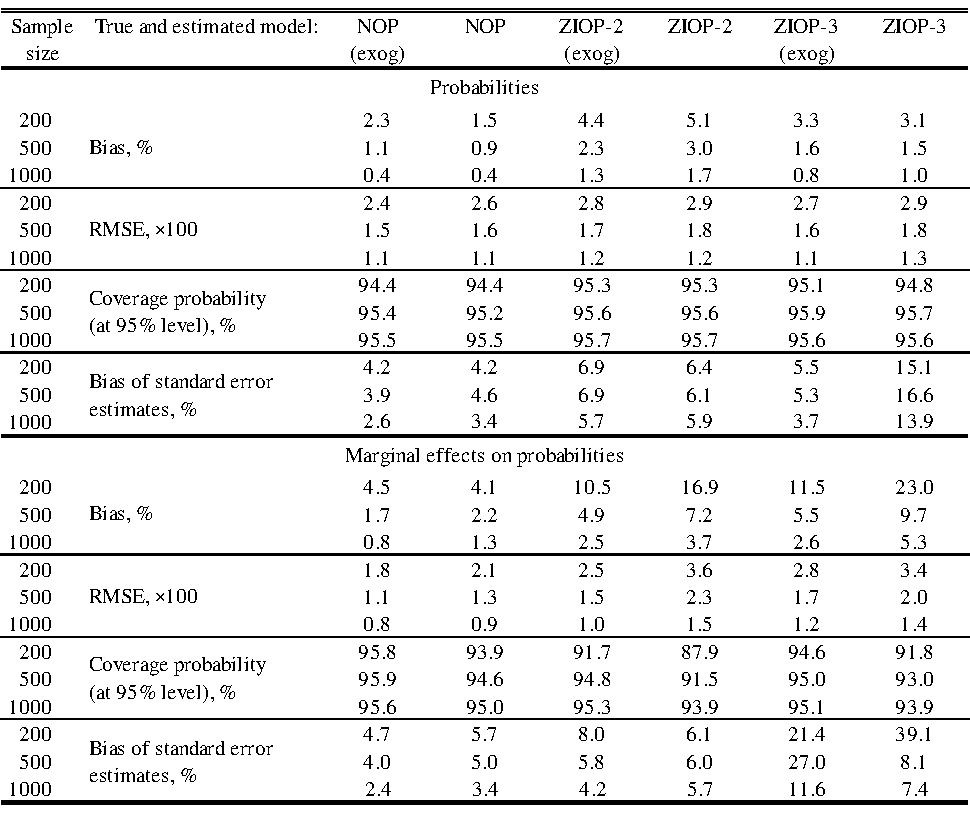
\includegraphics[
natheight=5.2154in, natwidth=6.2075in, height=5.2453in, width=6.2349in]
{C:/Users/user/Documents/Dale/Our paper on Github/cnop/paper/graphics/P6BDD601__2.pdf}%
%EndExpansion
\end{center}

%TCIMACRO{\TeXButton{TeX field}{\justify}}%
%BeginExpansion
\justify%
%EndExpansion
%TCIMACRO{\TeXButton{TeX field}{\footnotesize}}%
%BeginExpansion
\footnotesize%
%EndExpansion

Notes: (exog) -- exogenous switching; Bias -- the absolute difference
between the estimated and true values, devided by the true value; RMSE --
the absolute root mean square error of the estimates; Coverage probability
-- the percentage of times the estimated asymptotic 95\% confidence
intervals cover the true values; Bias of standard error estimates -- the
absolute difference between the average of the estimated asymptotic standard
errors of the estimates and the standard deviation of the estimates in all
replications. The above measures are averaged across five outcome
categories, and for the estimates of the MEs are also averaged across all
covariates.

%TCIMACRO{\TeXButton{E}{\end{table}}}%
%BeginExpansion
\end{table}%
%EndExpansion
%TCIMACRO{\TeXButton{Onehalf}{\begin{onehalfspace}}}%
%BeginExpansion
\begin{onehalfspace}%
%EndExpansion

\section{Application}

\section{\noindent \noindent Concluding remarks}

\section{Acknowledgments}

We gratefully acknowledge support from the Basic Research Program of the
National Research University Higher School of Economics, Moscow.

%TCIMACRO{\TeXButton{Single}{\end{onehalfspace}}}%
%BeginExpansion
\end{onehalfspace}%
%EndExpansion

\noindent

\begin{thebibliography}{99}
\bibitem{} Andrews, D. W. K. 2001. Testing when a parameter is on the
boundary of the maintained hypothesis.\ \textit{Econometrica} 69 (3):
683--734.

\bibitem{} Bagozzi, B. E., and B. Mukherjee. 2012. A mixture model for
middle category inflation in ordered survey responses.\ \textit{Political
Analysis\ }20: 369--386.

\bibitem{} Basu, D., and R. M. de Jong. 2007. Dynamic multinomial ordered
choice with an application to the estimation of monetary policy rules.\ 
\textit{Studies in Nonlinear Dynamics and Econometrics} 11 (4): 1--35.

\bibitem{} Brooks, R., M. N. Harris, and C. Spencer. 2012. Inflated ordered
outcomes.\ \textit{Economics Letters} 117 (3): 683--686.

\bibitem{} Famoye, F., and K. P. Singh. 2003. On inflated generalized
Poisson regression models. \textit{Advanced Applied Statistics} 3 (2):
145--158.

\bibitem{} Greene, W. H. 1994. Accounting for excess zeros and sample
selection in Poisson and negative binomial regression models.\ Working Paper
No. 94-10, Department of Economics, Stern School of Business, New York
University.

\bibitem{} Greene, W. H., and D. A. Hensher. 2010. \textit{Modeling ordered
choices: A primer}.\ Cambridge University Press.

\bibitem{} Harris, M. N., and X. Zhao. 2007. A zero-inflated ordered probit
model, with an application to modelling tobacco consumption.\ \textit{%
Journal of Econometrics} 141 (2): 1073--1099.

\bibitem{} Hartman, R. S., M. Doane, and C.-K. Woo. 1991. Consumer
rationality and the status quo.\ \textit{Quarterly Journal of Economics}
106: 141--162.

\bibitem{} Heckman, J. J. 1978. Dummy endogenous variables in a simultaneous
equation system. \textit{Econometrica} 46: 931--959.

\bibitem{} Hern\'{a}ndez, A., F. Drasgow and V. Gonz\'{a}les-Rom\'{a}. 2004.
Investigating the functioning of a middle category by means of a
mixed-measurement model. \textit{Journal of Applied Psychology} 89 (4):
687-699.

\bibitem{} Kahneman, D., J. L. Knetsch, and R. H. Thaler. 1991. Anomalies:
the endowment effect, loss aversion, and status quo bias.\ \textit{Journal
of Economic Perspectives} 5 (1): 193--206.

\bibitem{} Kelley, M. E., and S. J. Anderson. 2008. Zero inflation in
ordinal data: incorporating susceptibility to response through the use of a
mixture model.\ \textit{Statistics in Medicine} 27: 3674--3688.

\bibitem{} Kulas, J. T. and A. A. Stachowski. 2009. Middle category
endorsement in odd-numbered Likert response scales: Associated item
characteristics, cognitive demands, and preferred meanings. \textit{Journal
of Research in Personality }43: 489-493.

\bibitem{} Lambert, D. 1992. Zero-inflated Poisson regression with an
application to defects in manufacturing.\ \textit{Technometrics} 34 (1):
1--14.

\bibitem{} MacKinnon, J. G. 1996. Numerical distribution functions for unit
root and cointegration tests.\ \textit{Journal of Applied Econometrics} 11:
601--618.

\bibitem{} Samuelson, W., and R. Zeckhauser. 1988. Status quo bias in
decision making.\ \textit{Journal of Risk and Uncertainty} 1: 7--59.

\bibitem{} Sirchenko, A. 2013. A model for ordinal responses with an
application to policy interest rate. National Bank of Poland Working Paper
No. 148.

\bibitem{} Small, K. 1987. A discrete choice model for ordered
alternatives.\ \textit{Econometrica} 55: 409--424.

\bibitem{} Vovsha, P. 1997. Application of cross-nested logit model to mode
choice in Tel Aviv, Israel, Metropolitan Area.\ \textit{Transportation
Research Record} 1607: 6--15.

\bibitem{} Vuong, Q. 1989. Likelihood ratio tests for model selection and
non-nested hypotheses.\ \textit{Econometrica} 57 (2): 307--333.

\bibitem{} Wen, C.-H., and F. Koppelman. 2001. The generalized nested logit
model. \textit{Transportation Research B} 35: 627--641.

\bibitem{} Wilde, J. 2000. Identification of multiple equation probit models
with endogenous dummy regressors.\ \textit{Economics Letters} 69 (3):
309--312.

\bibitem{} Winkelmann, R. 2008. \textit{Econometric analysis of count data}%
.\ 5$^{\text{th}}$ edition, Springer.
\end{thebibliography}

\section*{Appendix}

% Table generated by Excel2LaTeX from sheet 'params'

%TCIMACRO{%
%\TeXButton{A}{\setcounter{table}{0}
%\renewcommand{\thetable}{A\arabic{table}}}}%
%BeginExpansion
\setcounter{table}{0}
\renewcommand{\thetable}{A\arabic{table}}%
%EndExpansion
%TCIMACRO{%
%\TeXButton{B}{\begin{table}[H] \captionsetup{singlelinecheck = false, justification=justified}}}%
%BeginExpansion
\begin{table}[H] \captionsetup{singlelinecheck = false, justification=justified}%
%EndExpansion

\caption{Monte Carlo simulations: The true values of parameters\label{True
param}}%
%TCIMACRO{\TeXButton{TeX field}{\centering}}%
%BeginExpansion
\centering%
%EndExpansion

\begin{center}
%TCIMACRO{%
%\FRAME{itbpF}{6.4284in}{2.6766in}{0in}{}{}{Figure}{%
%\special{language "Scientific Word";type "GRAPHIC";maintain-aspect-ratio TRUE;display "USEDEF";valid_file "T";width 6.4284in;height 2.6766in;depth 0in;original-width 6.4001in;original-height 2.6484in;cropleft "0";croptop "1";cropright "1";cropbottom "0";tempfilename 'P6TXE50A.wmf';tempfile-properties "XPR";}}}%
%BeginExpansion
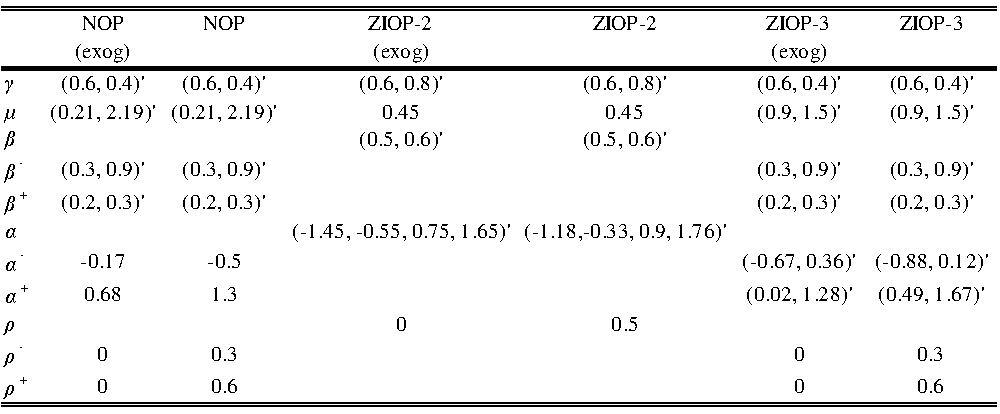
\includegraphics[
natheight=2.6484in, natwidth=6.4001in, height=2.6766in, width=6.4284in]
{C:/Users/user/Documents/Dale/Our paper on Github/cnop/paper/graphics/P6TXE50A__3.pdf}%
%EndExpansion
\end{center}

%TCIMACRO{\TeXButton{TeX field}{\justify}}%
%BeginExpansion
\justify%
%EndExpansion
%TCIMACRO{\TeXButton{TeX field}{\footnotesize}}%
%BeginExpansion
\footnotesize%
%EndExpansion

Notes: (exog) -- exogenous switching; the variances $\sigma ^{2},$ $\sigma
_{-}^{2},$ $\sigma _{+}^{2},$ and $\sigma _{\nu }^{2}$ are all fixed to one.

%TCIMACRO{\TeXButton{E}{\end{table}}}%
%BeginExpansion
\end{table}%
%EndExpansion

\end{document}
